% Compile with XeLaTeX. All included tables and figures are local to this folder.
\documentclass[11pt,a4paper]{article}
\usepackage[margin=23mm,headheight=15pt]{geometry}
\usepackage{fontspec}
\setmainfont{Latin Modern Roman}
\setsansfont{Latin Modern Sans}
\setmonofont{Latin Modern Mono}[Scale=MatchLowercase]
\usepackage{amsmath,amssymb,graphicx,booktabs,longtable,array}
\usepackage{xcolor}
\definecolor{ink}{HTML}{17324D}
\definecolor{linkblue}{HTML}{1E5A85}
\usepackage[font=small,labelfont=bf,justification=raggedright,singlelinecheck=false]{caption}
\usepackage{fancyhdr}
\usepackage{placeins}
\usepackage{ragged2e}
\usepackage{xurl}
\usepackage[unicode,colorlinks=true,linkcolor=linkblue,citecolor=linkblue,urlcolor=linkblue,
 pdftitle={Inferring Cosmological Parameters from Simulated Matter Density Fields},
 pdfauthor={CSCI 494 Project Team}]{hyperref}
\pagestyle{fancy}
\fancyhf{}
\fancyhead[L]{\small\sffamily COSMOREG\quad Project report v1}
\fancyhead[R]{\small\sffamily CSCI 494}
\fancyfoot[C]{\thepage}
\renewcommand{\headrulewidth}{0.3pt}
\setlength{\parindent}{0pt}
\setlength{\parskip}{5pt plus 1pt}
\setlength{\emergencystretch}{3em}
\setcounter{tocdepth}{1}
\renewcommand{\arraystretch}{1.15}
\newcommand{\Om}{\Omega_{\mathrm m}}
\newcommand{\sig}{\sigma_8}
\newcommand{\model}[1]{\texttt{\detokenize{#1}}}
\newcommand{\sourcecommit}{64e6cecd8869}


\begin{document}
\raggedright
\begin{titlepage}
\vspace*{18mm}
{\Large\sffamily\color{ink} CSCI 494\quad /\quad PROJECT REPORT}\par
\vspace{12mm}
{\Huge\bfseries\color{ink} Inferring Cosmological\\Parameters from Simulated\\Matter Density Fields\par}
\vspace{7mm}
{\Large Ridge regression, multilayer perceptrons, convolutional networks, and Gaussian-noise experiments}\par
\vspace{14mm}
{\large CSCI 494 Project Team}\par
{\large Report version 1\quad |\quad 12 November 2026}\par
\vspace{12mm}
\hrule
\vspace{5mm}
\textbf{Evidence snapshot.} This report consolidates the saved experiment results and graphs in the merged \texttt{cosmoreg} repository at commit \texttt{\sourcecommit}. It contains all 243 saved CNN validation scores, all nine MLP configuration summaries and 45 associated fold experiments, the Ridge and MLP test results at three dataset levels, the common level-3 model comparison, and every saved raster graph, including distinct notebook renderings.

\textbf{Reporting scope.} Numerical tables are transcribed or generated from existing CSV, JSON, and notebook outputs. No training or new test-set evaluation was performed to prepare this report. Recomputed errors from saved prediction arrays were used only to check the transcription.
\vfill
\textbf{Main finding.} On the common clean level-3 test set, the best recorded map-level RMSE is 0.0192 for $\Om$ (16-step CNN) and 0.0304 for $\sig$ (10-step CNN), compared with baseline errors of 0.1198 and 0.1124. These are point estimates from the saved runs, rather than uncertainty estimates or claims about other simulation suites.
\end{titlepage}

\begin{abstract}
We study supervised estimation of the matter-density parameter $\Om$ and fluctuation-amplitude parameter $\sig$ from CAMELS IllustrisTNG total-matter maps at redshift zero. The project compares Ridge regression and a multilayer perceptron (MLP) on 50-bin projected power spectra with convolutional neural networks (CNNs) on full $256\times256$ density maps. Simulation-level partitioning keeps each simulation's 15 related maps together across training, validation, and test groups. The three disjoint dataset levels contain 67, 333, and 600 simulations. Ridge and MLP tests show moderate gains over a training-mean baseline, with weak small-sample performance for $\sig$. On the level-3 held-out test set of 120 simulations and 1,800 maps, the 10-step CNN obtains map RMSE $(0.0211,0.0304)$ and the 16-step CNN obtains $(0.0192,0.0324)$ for $(\Om,\sig)$. Averaging predictions within each simulation improves these errors further, though the two CNNs retain different strengths. Saved Gaussian-noise experiments show larger group-average errors at noise strength 0.05 than at 0.01. Because those experiments use corrupted training and test inputs, different shortlisted models, and validation-selected checkpoints, they do not establish the benefit of training-time augmentation on clean data. Complete score tables, all saved figures, and a source manifest accompany this report.
\end{abstract}

\begingroup
\small\setlength{\parskip}{0pt}
\tableofcontents
\endgroup
\clearpage

\section{Introduction and research questions}
The project asks how well simulated matter-density fields constrain two cosmological parameters, and how performance changes when the input is compressed into a power spectrum. CAMELS was designed to support joint studies of cosmology and astrophysics with varied simulation parameters \cite{camels,cmd}. Here, $\Om$ denotes the present-day matter-density fraction, and $\sig$ is the amplitude of linear matter fluctuations on the conventional $8\,h^{-1}\,\mathrm{Mpc}$ scale. The task is supervised point prediction within the IllustrisTNG Latin-hypercube (LH) dataset.

Three comparisons guide the analysis. First, does a nonlinear MLP improve on a regularized linear predictor when both receive the same 50 spectral features? Second, how much predictive accuracy is obtained by giving a CNN access to the full spatial field? Third, what do the saved noise experiments reveal about performance on corrupted maps? The final comparison uses the same level-3 test simulations for all four principal models. Results from other levels and the complete validation search remain part of the record, rather than being replaced by the best final result.

The repository README describes an earlier preprocessing-only scope. This report follows the merged implementation and saved model outputs, which also include training and evaluation. The relevant local evidence is identified throughout and frozen under \path{sources/}; its original repository paths and SHA-256 hashes are listed in \path{source_manifest.json} \cite{repo}.

\section{Dataset and preprocessing}
\subsection{Source data and targets}
The configured input is \path{Maps_Mtot_IllustrisTNG_LH_z=0.00.npy}, paired with \path{params_LH_IllustrisTNG.txt}. The project uses 1,000 LH simulations and 15,000 total-matter maps. Each map has $256^2$ pixels and spans a periodic square of side $25\,h^{-1}\,\mathrm{Mpc}$ at $z=0$; these geometric properties match the CMD documentation \cite{docs}. Fifteen consecutive maps belong to one simulation, so map index $i$ is associated with parameter row $\lfloor i/15\rfloor$ in the project's loader.

The first two columns of the parameter file provide $\Om$ and $\sig$. Four additional supernova and active-galactic-nucleus feedback parameters are retained as metadata, but are not regression targets. The learned mapping therefore operates across the astrophysical variations present in this dataset. This should not be interpreted as a demonstration of transfer to observations or to a different hydrodynamical simulator.

\subsection{Simulation-grouped partitioning}
\path{camels_pipeline/splits.py} shuffles simulation IDs with seed 42, partitions them into three \emph{disjoint} levels, and assigns complete simulations to a held-out test group and five development folds. It audits overlap both within and across levels. The counts in Table~\ref{tab:splits} follow the actual split contract, which rounds the requested map counts to whole simulations.

\begin{table}[htbp]\centering\small
\caption{Dataset sizes. Development means the union of folds 1--5; fold sizes are counts of simulations.}\label{tab:splits}
\begin{tabular}{lrrrrrl}
\toprule
Level & All sims & All maps & Dev sims & Dev maps & Test maps & Dev fold sims\\
\midrule
1 & 67 & 1,005 & 54 & 810 & 195 & 11, 11, 11, 11, 10\\
2 & 333 & 4,995 & 266 & 3,990 & 1,005 & 54, 53, 53, 53, 53\\
3 & 600 & 9,000 & 480 & 7,200 & 1,800 & 96, 96, 96, 96, 96\\
\bottomrule
\end{tabular}
\end{table}

The test groups contain 13, 67, and 120 simulations, respectively. Splitting individual maps at random would allow related views of the same simulated universe to appear on both sides of evaluation. The grouped scheme avoids that failure. Because the levels are disjoint rather than nested, their score differences combine changes in sample size with changes in the actual cosmologies assigned to training and test sets. Plots against development size are descriptive comparisons, not a controlled learning-curve experiment.

\subsection{Projected power-spectrum features}
For a raw density map $\rho$, the preprocessing pipeline forms the dimensionless density contrast
\begin{equation}
\delta(\mathbf{x})=\frac{\rho(\mathbf{x})}{\langle\rho\rangle}-1
\end{equation}
before any learned normalization. Using NumPy's unnormalized two-dimensional FFT, the saved convention is
\begin{equation}
P_{\mathrm{2D}}(\mathbf{k})=\frac{L^2}{N^4}\left|\operatorname{FFT}_2[\delta](\mathbf{k})\right|^2,
\qquad L=25\,\mathrm{Mpc}/h,\quad N=256.
\end{equation}
The DC mode is excluded. Fifty fixed linear radial bins run from $2\pi/L$ through the axis Nyquist frequency $\pi N/L$; modes above that axis limit are omitted. The saved representative $k$ is the mean mode magnitude within each bin. Features are $\log_{10}\max(P,10^{-30})$ for the MLP. Ridge applies $\log_{10}$ to the positive raw spectra within its pipeline. The saved Ridge sanity-check output reports strictly positive spectra for every level. This statistic is the project's projected 2D spectrum, not a supplied 3D matter spectrum.

Paired map and spectrum exports contain labels, simulation IDs, map IDs, and manifests. The software checks row alignment and simulation isolation. Those implementation checks establish the intended data handling; they do not independently reproduce every historical model run summarized here.

\subsection{CNN input transformation}
CNN inputs use $\log_{10}\max(\rho,10^{-5})$, followed by one global training-set mean and standard deviation over all training pixels. The resulting tensor has shape $(M,1,256,256)$. During validation search, these statistics are fitted using folds 1--4 and reused for fold 5. During final clean CNN training, the statistics are refitted using all five development folds and stored with the checkpoint. CNN targets remain in their original units.

\section{Models and experimental protocol}
\subsection{Ridge regression baseline}
The Ridge notebook composes logarithmic features, \texttt{StandardScaler}, and \texttt{Ridge} in one scikit-learn pipeline. For each target it minimizes squared residuals with an $\ell_2$ coefficient penalty,
\begin{equation}
\min_{\mathbf w,b}\sum_i(y_i-\mathbf w^\mathsf T\mathbf z_i-b)^2+\alpha\|\mathbf w\|_2^2,
\end{equation}
where $\mathbf z$ is the standardized log spectrum. The scaler is fitted inside each training split. Forty-one regularization strengths from $10^{-6}$ to $10^4$ are assessed with five-fold grouped cross-validation. Mean fold RMSE selects $\alpha$ independently for each target. A final model is fitted on all development folds and evaluated on the test group.

\subsection{Multilayer perceptron}
The spectral MLP has two ReLU hidden layers and a linear two-output layer. The original and stronger-decay configurations use $50\rightarrow32\rightarrow16\rightarrow2$ (2,194 trainable parameters); the larger configuration uses $50\rightarrow64\rightarrow32\rightarrow2$ (5,410 parameters). Both features and targets are standardized using training data only. Reported physical-unit predictions invert the target standardization.

All three configurations use AdamW with learning rate $10^{-3}$, batch size 64, and a maximum of 20 development epochs. The original and larger networks use weight decay $10^{-4}$; stronger decay uses $10^{-2}$. Weight initialization and the comparison batch-order generator use seed 42. The best validation-MSE epoch is retained within each fold.

Configuration selection uses simulation-level errors pooled across held-out development folds:
\begin{equation}
S=\frac12\sum_{t\in\{\Om,\sig\}}
\frac{\mathrm{RMSE}_{t,\mathrm{pooled}}}{\mathrm{RMSE}_{t,\mathrm{baseline,pooled}}}.
\end{equation}
The final epoch count is the median of the five selected development epochs. The fixed architecture, scalers, and weights are then fitted on the entire development set without test-driven checkpoint selection. The chosen settings are larger/11 epochs for level 1, stronger decay/13 epochs for level 2, and larger/12 epochs for level 3. The MLP test snapshots record evaluation dates of 12 October 2026 for level 1 and 13 October 2026 for levels 2 and 3.

\subsection{CNN architecture search and final models}
The registry contains 40 CNN variants: five variants each at step labels 4, 6, 8, and 10, six at labels 12 and 14, and eight at label 16. These numbers are the authors' \emph{operation-step labels}, which count activations and pooling as well as learned operations; they are not counts of convolutional layers. The two tagged clean searches each contain 20 models at level 1, ten at level 2, and five at level 3. The level runner ranks the previous level before selecting the next shortlist.

The validation training code uses folds 1--4 for training and fold 5 for validation, MSE averaged across the two unscaled targets, AdamW at learning rate $3\times10^{-4}$ and weight decay $10^{-4}$, batch size 32, gradient clipping at norm 1, and cosine annealing toward $10^{-5}$ over 25 epochs. The minimum validation-MSE checkpoint is saved. This is a single validation fold, rather than the five-fold protocol used for Ridge and MLP.

The final clean comparison fixes \model{model_10_5} and \model{model_16_5}, the level-3 winners of the two tagged searches, and trains each for 25 epochs on all 7,200 development maps. The final epoch is retained without validation selection. Their structures are:
\begin{itemize}
\item \textbf{CNN-10:} three $3\times3$ convolutional blocks with 64, 128, and 256 output channels and LeakyReLU activations. Two $4\times4$ max-pooling operations are followed by adaptive average pooling to $2\times2$ and a linear $1024\rightarrow2$ head.
\item \textbf{CNN-16:} five convolutions with output channels 32, 64, 128, 128, and 128, using kernel sizes 5, 5, 7, 3, and 3. The network includes two batch-normalization layers, LeakyReLU, two $4\times4$ max-pooling operations, adaptive average pooling to $2\times2$, and a $512\rightarrow32\rightarrow2$ head.
\end{itemize}
The final checkpoint payload includes preprocessing statistics, training simulation IDs, settings, and target means. The test notebook checks that those training IDs do not overlap its test IDs.

\subsection{Gaussian-noise experiments}
For map $\rho_m$, the saved augmentation code constructs
\begin{equation}
\widetilde\rho_m(\mathbf{x})=
\max\!\left(0,\rho_m(\mathbf{x})+\alpha s_m\epsilon_m(\mathbf{x})\right),
\quad \epsilon_m(\mathbf{x})\sim\mathcal N(0,1),
\end{equation}
where $s_m$ is the spatial standard deviation of that raw map. The noise strengths are $\alpha=0.01$ and $0.05$. The transform preserves float32 shape and labels, and clips negative densities before the CNN logarithm. It creates one deterministic corrupted copy of each map; it does not expand the number of training examples or sample fresh noise every epoch.

The generator visits every \path{maps.npy} leaf, including test leaves, and initializes the same random seed for each leaf. Consequently, these experiments evaluate networks trained and tested at the matching corruption setting. Reusing the seed can repeat corresponding noise patterns across equal-shaped leaves and merits revision in a future robustness study. Metadata and manifests are copied from the clean data rather than updated with a new corruption provenance record.

The noise test notebook evaluates five shortlisted checkpoints per group: step labels 4--10 (group 1) and 12--16 (group 2). It computes the arithmetic mean of the five separate model MAEs and RMSEs. It does \emph{not} average predictions into an ensemble. Preprocessing statistics use folds 1--4, consistent with the saved validation-selected checkpoints; unlike the final clean CNNs, these models are not refitted on all five development folds. Model membership also changes between noise settings. These distinctions limit direct comparisons with the clean final test.

\section{Evaluation definitions}
For one target, map-level errors use every test map:
\begin{equation}
\mathrm{MAE}=\frac1M\sum_{i=1}^M|\hat y_i-y_i|,
\qquad
\mathrm{RMSE}=\sqrt{\frac1M\sum_{i=1}^M(\hat y_i-y_i)^2}.
\end{equation}
Simulation-level evaluation first averages the 15 predictions from each simulation,
\begin{equation}
\overline{\hat y}_s=\frac1{15}\sum_{i\in s}\hat y_i,
\end{equation}
then computes errors across the test simulations. The true target is constant within a simulation. This averaging uses multiple views, so it represents a different inference setting from prediction using a single map.

The baseline always predicts the target mean of the development training set. A reported RMSE reduction is $100(1-\mathrm{RMSE}_{\mathrm{model}}/\mathrm{RMSE}_{\mathrm{baseline}})$ percent. Negative values mean worse performance than that baseline. Ridge also reports $R^2$ relative to the test-target mean. All RMSE and MAE values in the test tables are in original parameter units.

MLP training/validation losses use standardized targets, whereas CNN validation losses use unscaled targets. Their MSE magnitudes therefore cannot be used to rank the two model families. The common final comparison instead uses the same held-out maps and physical-unit metrics. Map errors are correlated within simulations; 1,800 maps should not be treated as 1,800 independent universes when estimating uncertainty.

\section{Results: spectral models}
\subsection{Ridge cross-validation and tests}
The selected regularization grows from $(100,100)$ at level 1 to approximately $(177.828,316.228)$ at level 3, in target order $(\Om,\sig)$. The saved cross-validation summaries are given in Table~\ref{tab:ridge-cv}, and the full test metrics in Table~\ref{tab:ridge}. The regularization curves in Figure~\ref{fig:ridge-cv} flatten over much of the grid, especially at larger levels.

\begin{table}[htbp]\centering\small
\caption{Ridge five-fold validation summaries transcribed at the precision printed in the saved notebook. Values after $\pm$ are fold standard deviations, not confidence intervals.}\label{tab:ridge-cv}
\begin{tabular}{llrrr}
\toprule
Level & Target & Selected $\alpha$ & CV RMSE & CV MAE\\
\midrule
1 & $\Om$ & 100 & $0.0953\pm0.0157$ & $0.0816\pm0.0171$\\
1 & $\sig$ & 100 & $0.0977\pm0.0170$ & $0.0826\pm0.0155$\\
2 & $\Om$ & 100 & $0.0896\pm0.0055$ & $0.0743\pm0.0055$\\
2 & $\sig$ & 177.828 & $0.0956\pm0.0045$ & $0.0792\pm0.0047$\\
3 & $\Om$ & 177.828 & $0.0919\pm0.0034$ & $0.0755\pm0.0027$\\
3 & $\sig$ & 316.228 & $0.0989\pm0.0043$ & $0.0832\pm0.0031$\\
\bottomrule
\end{tabular}
\end{table}
\begingroup\footnotesize\setlength{\tabcolsep}{3pt}\renewcommand{\arraystretch}{1.05}
\begin{longtable}{lrrrrrrrrr}
\caption{Complete Ridge held-out test results in original units.}\label{tab:ridge}\\
\toprule
Level & Target & $\alpha$ & MAE & RMSE & $R^2$ & Sim MAE & Sim RMSE & Sim $R^2$ & Base RMSE \\
\midrule
\endfirsthead
\toprule
Level & Target & $\alpha$ & MAE & RMSE & $R^2$ & Sim MAE & Sim RMSE & Sim $R^2$ & Base RMSE \\
\midrule\endhead
\bottomrule\endfoot
1 & $\Omega_m$ & 100.000 & 0.1124 & 0.1266 & 0.2875 & 0.1116 & 0.1229 & 0.3285 & 0.1500 \\
1 & $\sigma_8$ & 100.000 & 0.0924 & 0.1072 & -0.0374 & 0.0876 & 0.0996 & 0.1056 & 0.1054 \\
2 & $\Omega_m$ & 100.000 & 0.0735 & 0.0869 & 0.4139 & 0.0678 & 0.0788 & 0.5177 & 0.1138 \\
2 & $\sigma_8$ & 177.828 & 0.0744 & 0.0934 & 0.2792 & 0.0690 & 0.0864 & 0.3827 & 0.1102 \\
3 & $\Omega_m$ & 177.828 & 0.0747 & 0.0925 & 0.3910 & 0.0675 & 0.0827 & 0.5130 & 0.1198 \\
3 & $\sigma_8$ & 316.228 & 0.0832 & 0.1000 & 0.1958 & 0.0780 & 0.0940 & 0.2888 & 0.1124 \\
\end{longtable}\endgroup


\begin{figure}[htbp]\centering
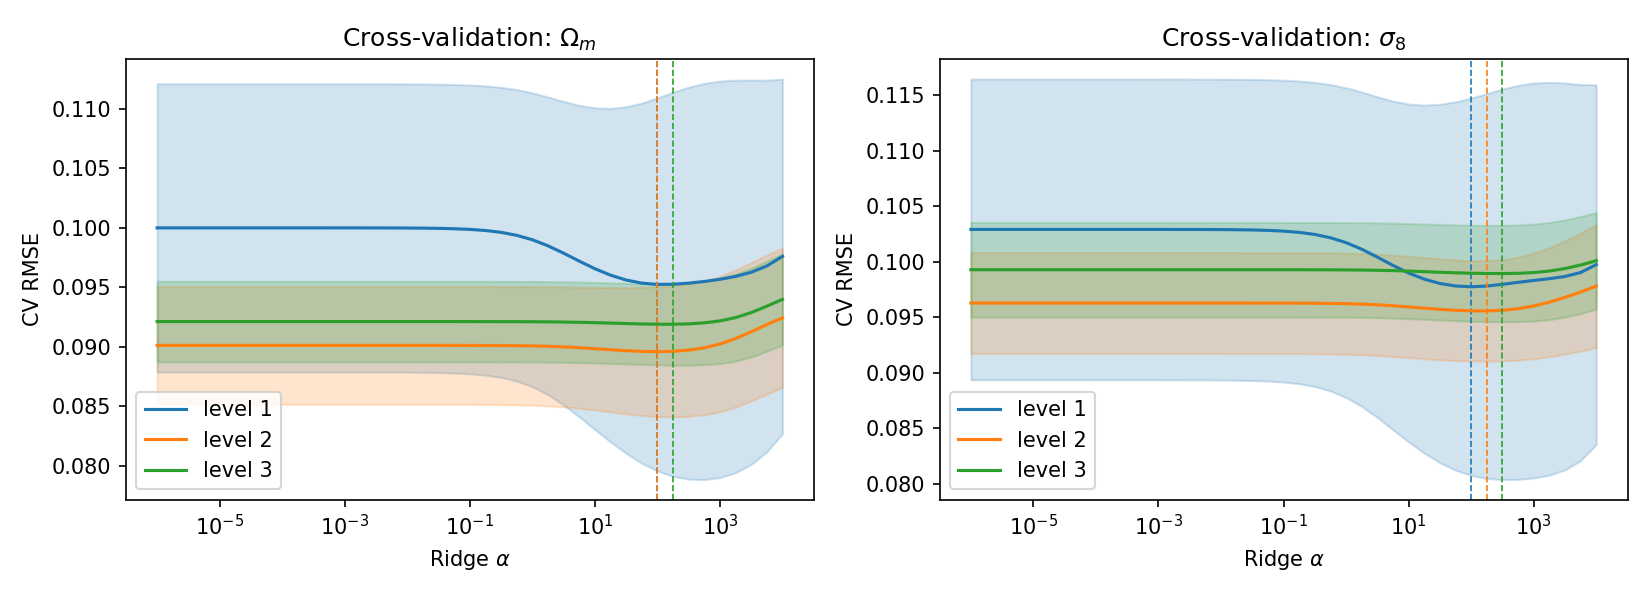
\includegraphics[width=\linewidth]{figures/ridge_cv.png}
\caption{Saved Ridge cross-validation curves for both targets. The source notebook supplies the numerical summaries in Table~\ref{tab:ridge-cv}.}\label{fig:ridge-cv}
\end{figure}

Ridge improves $\Om$ prediction over the training-mean baseline at every level. For $\sig$ at level 1, map RMSE is 0.1072 versus a baseline of 0.1054, and map $R^2=-0.0374$. The corresponding simulation-averaged RMSE is 0.0996. At levels 2 and 3 both target predictions improve on the map baseline. Level 2 has lower test RMSE than level 3 for both targets despite having fewer development maps. Because those tests use different simulation groups, this does not imply that increasing the size of a fixed training set worsens generalization.

\begin{figure}[p]\centering
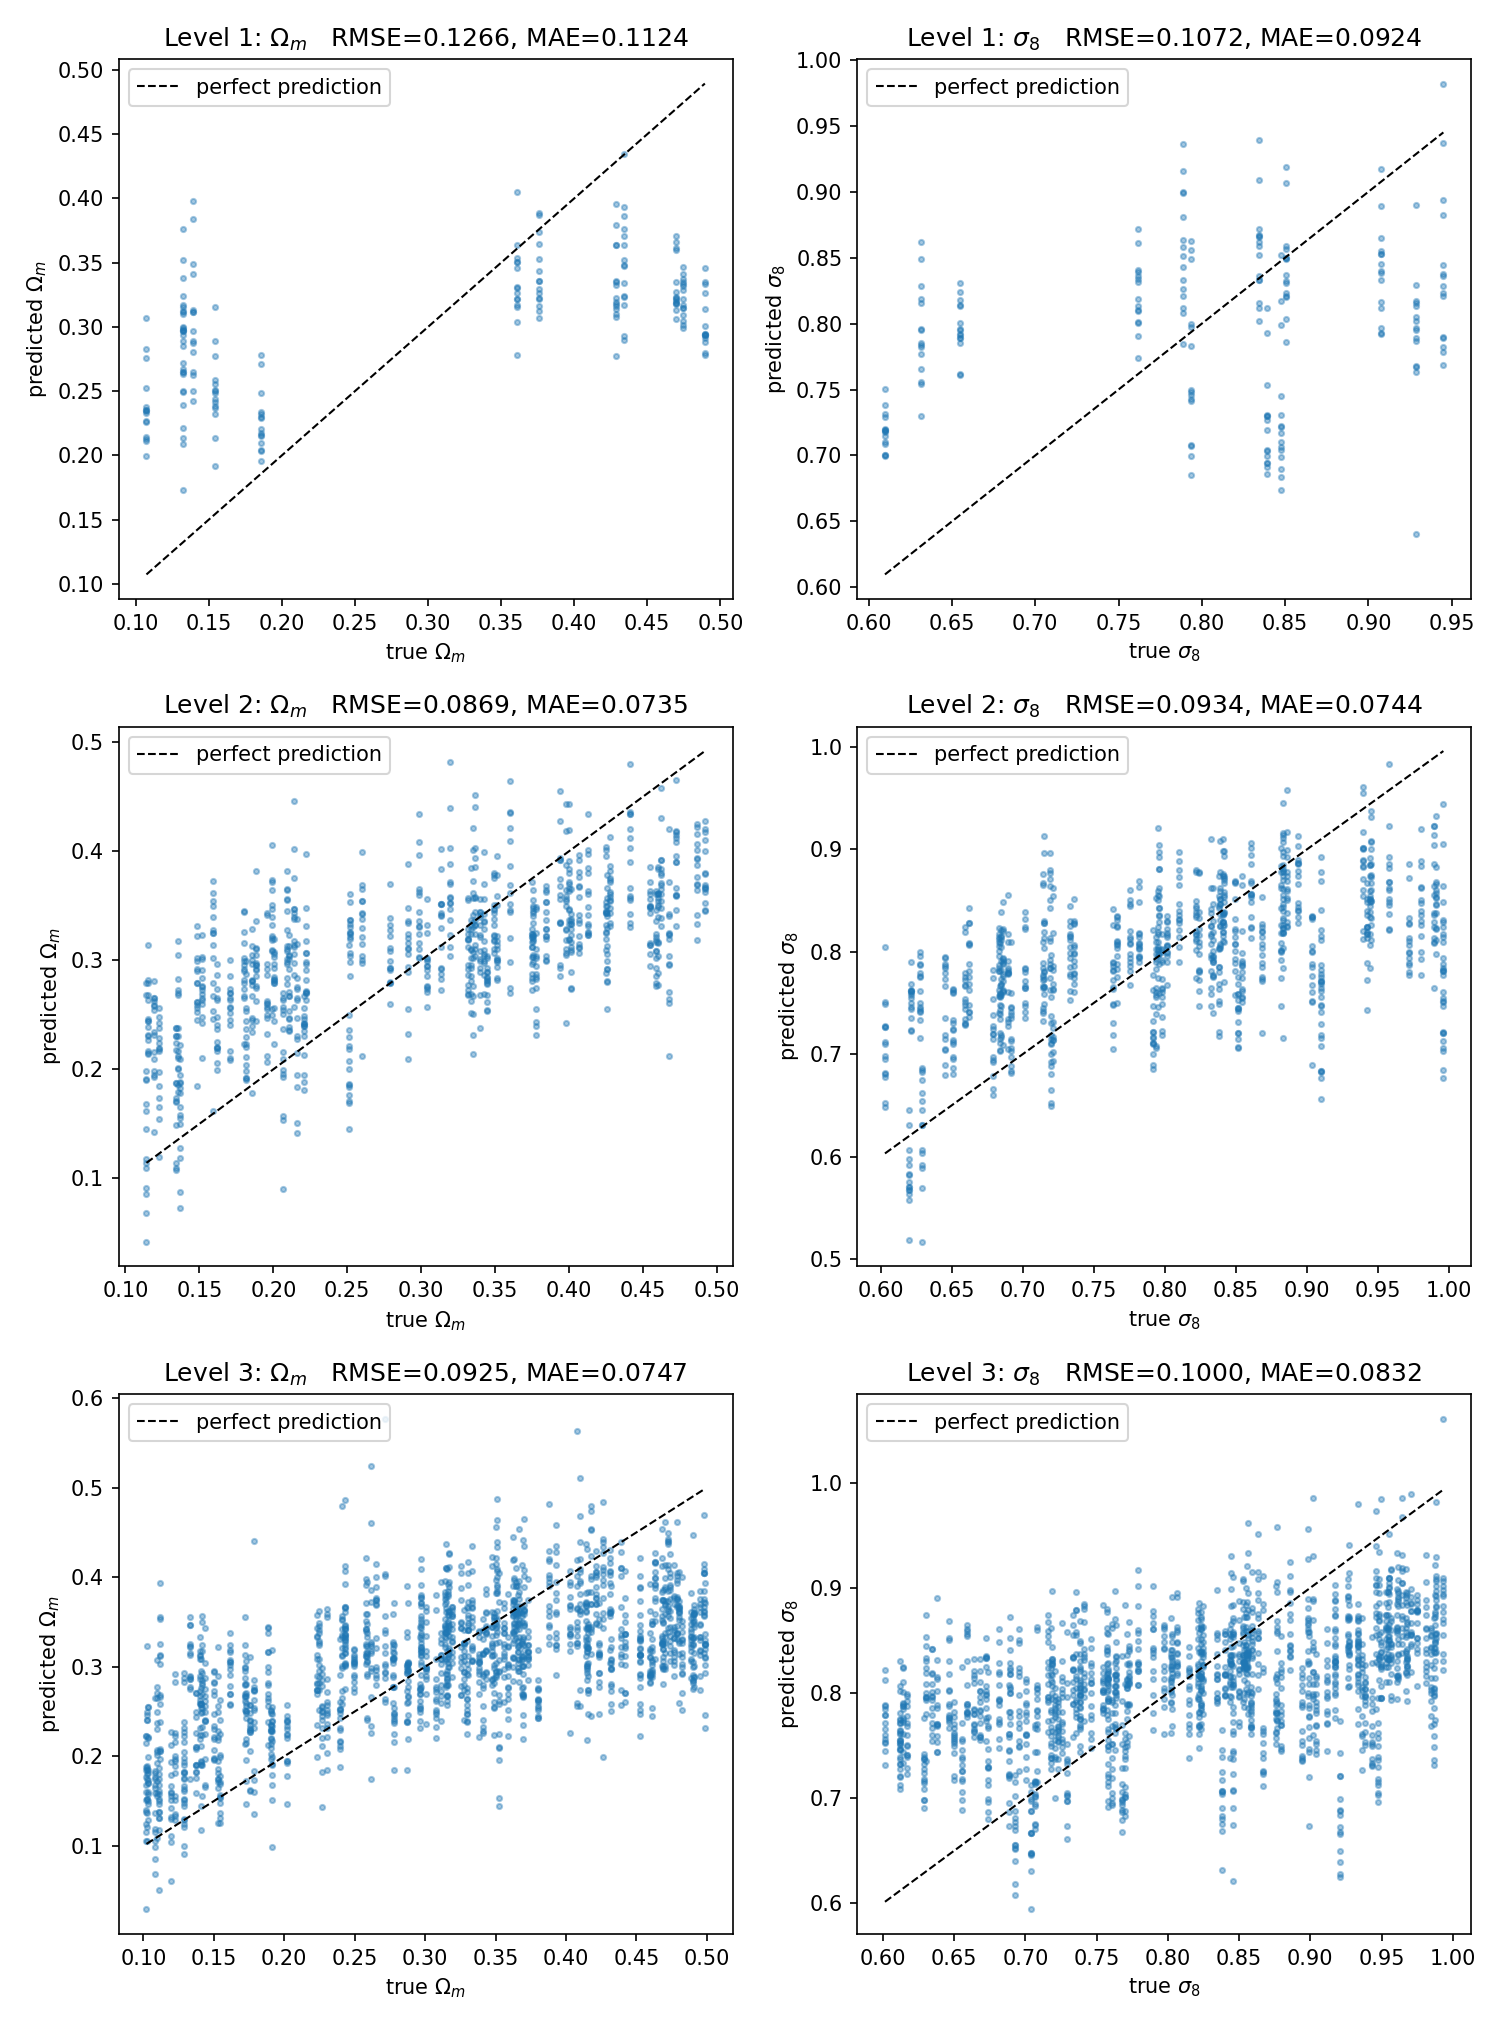
\includegraphics[width=.85\linewidth,height=.77\textheight,keepaspectratio]{figures/ridge_predictions.png}
\caption{Saved Ridge predicted-versus-true scatter plots for all three levels and both targets, scored per map. Related views share the same true target and form vertical bands.}\label{fig:ridge-pred}
\end{figure}
\begin{figure}[htbp]\centering
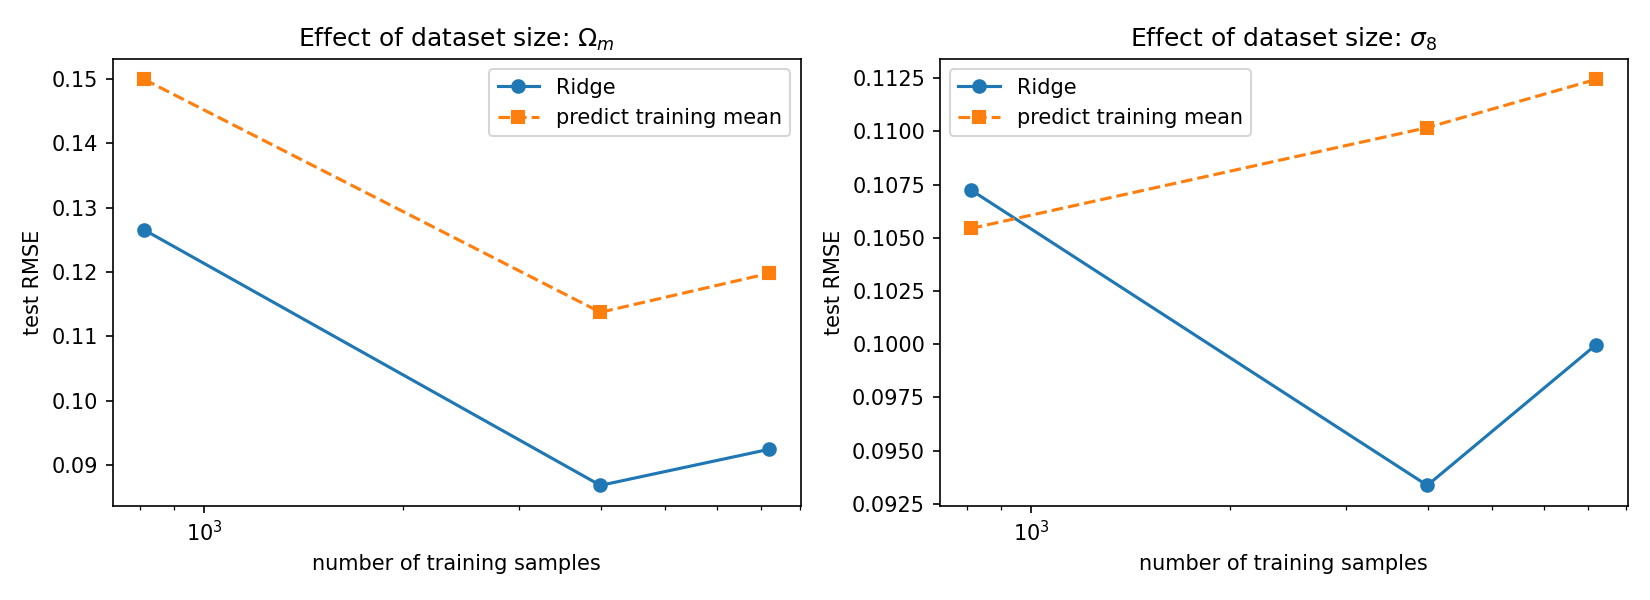
\includegraphics[width=\linewidth]{figures/ridge_size.png}
\caption{Saved Ridge test RMSE against development-map count. The x-axis changes both training size and the disjoint level-specific test group.}\label{fig:ridge-size}
\end{figure}
\FloatBarrier

\subsection{MLP development comparisons}
Table~\ref{tab:mlp-cv} includes every saved configuration summary. The larger MLP leads at levels 1 and 3, while stronger decay leads at level 2. At level 2 the leading scores, 0.693170 and 0.693320, are nearly identical; the ranking alone is not evidence of a robust advantage for stronger weight decay. At level 3 the larger network reaches pooled simulation RMSE $(0.0789,0.0852)$ in development. Fold RMSE standard deviations are larger at level 1, consistent with its much smaller validation groups.
\begingroup\footnotesize\setlength{\tabcolsep}{3pt}\renewcommand{\arraystretch}{1.05}
\begin{longtable}{lrrrrrrr}
\caption{All MLP configuration summaries. RMSE is pooled by simulation; SD is the fold RMSE standard deviation.}\label{tab:mlp-cv}\\
\toprule
Level & Configuration & Score & RMSE $\Omega_m$ & RMSE $\sigma_8$ & SD $\Omega_m$ & SD $\sigma_8$ & Best epochs \\
\midrule
\endfirsthead
\toprule
Level & Configuration & Score & RMSE $\Omega_m$ & RMSE $\sigma_8$ & SD $\Omega_m$ & SD $\sigma_8$ & Best epochs \\
\midrule\endhead
\bottomrule\endfoot
1 & original & 0.805545 & 0.0892 & 0.0900 & 0.0180 & 0.0188 & 9,17,18,11,20 \\
1 & larger & 0.795203 & 0.0869 & 0.0901 & 0.0175 & 0.0198 & 3,6,18,11,19 \\
1 & stronger\_decay & 0.806355 & 0.0893 & 0.0901 & 0.0179 & 0.0188 & 9,17,18,11,20 \\
2 & original & 0.693320 & 0.0782 & 0.0806 & 0.0056 & 0.0076 & 13,13,19,12,13 \\
2 & larger & 0.693837 & 0.0783 & 0.0806 & 0.0058 & 0.0080 & 17,13,17,5,13 \\
2 & stronger\_decay & 0.693170 & 0.0781 & 0.0806 & 0.0059 & 0.0075 & 13,13,19,11,13 \\
3 & original & 0.705331 & 0.0797 & 0.0856 & 0.0039 & 0.0043 & 12,18,16,9,17 \\
3 & larger & 0.699957 & 0.0789 & 0.0852 & 0.0050 & 0.0037 & 12,16,9,4,17 \\
3 & stronger\_decay & 0.705078 & 0.0796 & 0.0857 & 0.0034 & 0.0044 & 12,18,16,9,19 \\
\end{longtable}\endgroup


\begin{figure}[p]\centering
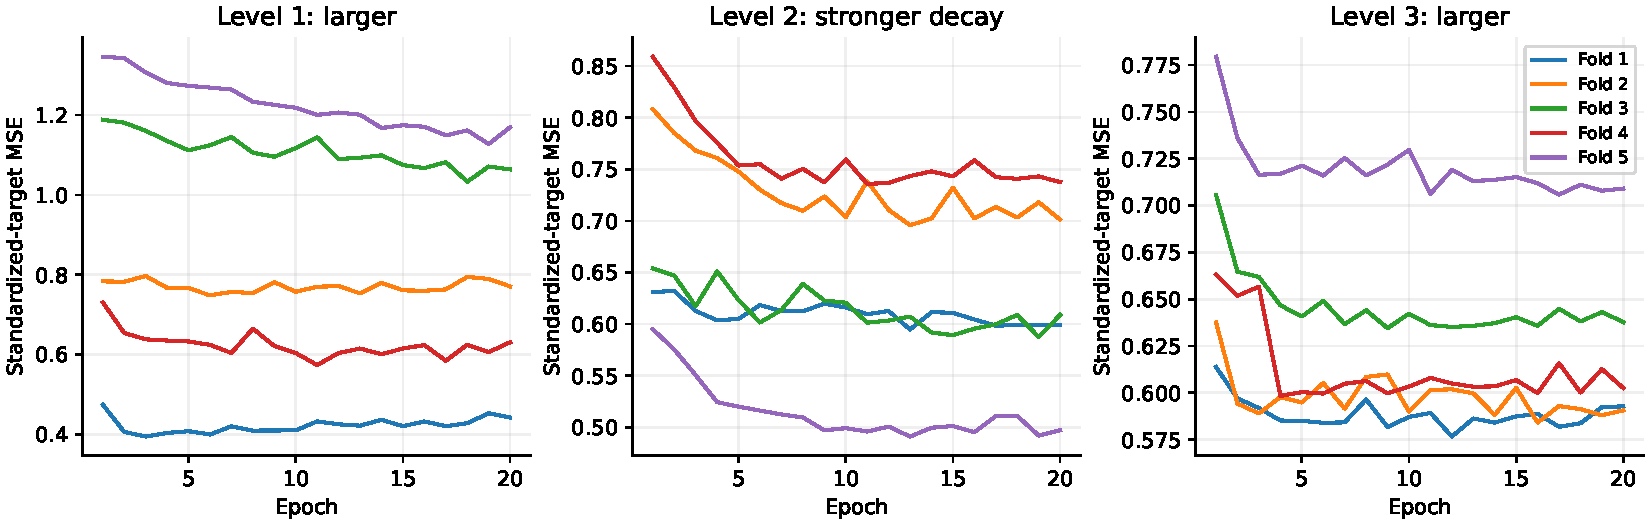
\includegraphics[width=\linewidth]{figures/mlp_fold_histories.pdf}
\caption{Validation histories for each level's selected MLP configuration, plotted from saved fold histories. These are standardized-target MSEs and are not directly comparable to CNN validation MSE.}\label{fig:mlp-folds}
\end{figure}

The initial level-1 notebook predates the configuration comparison. Its original $32,16$ network reached best validation epoch 18 on fold 5, with standardized validation MSE 1.1517 against baseline 1.2424. It reported map RMSE $(0.1192,0.1090)$ and simulation RMSE $(0.1155,0.1039)$. A subsequent five-fold run of that initial setup recorded pooled simulation RMSE $(0.0897,0.0902)$ and best epochs $(14,5,19,11,18)$. These preliminary outputs are preserved in the notebook snapshots. They are separate runs from the later controlled three-configuration comparison and from the final test model.

\begin{figure}[p]\centering
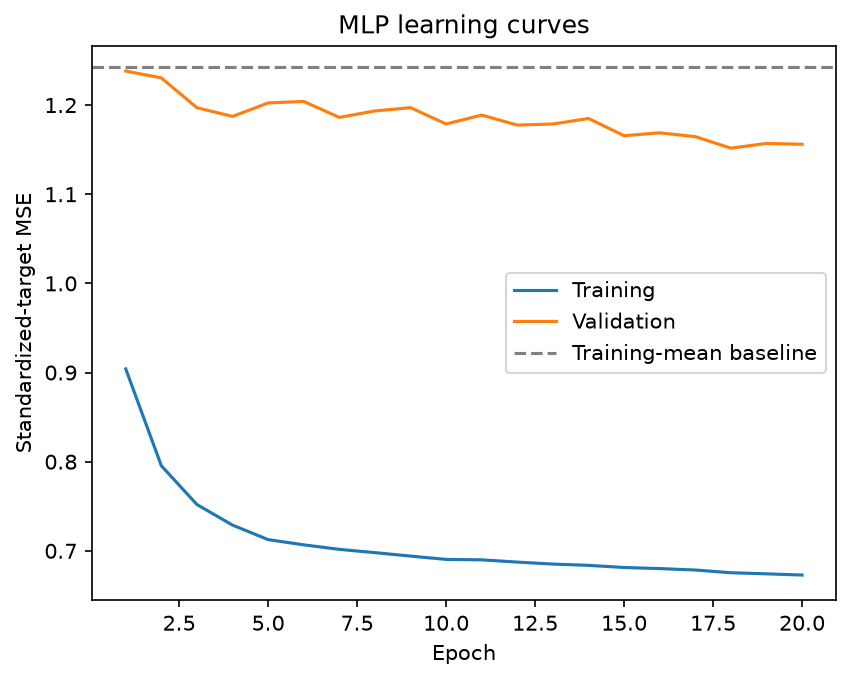
\includegraphics[width=.75\linewidth,height=.45\textheight,keepaspectratio]{figures/mlp_learning.png}
\caption{Original level-1 MLP learning curves from the saved preliminary validation notebook. Falling training loss with a much flatter validation curve indicates a persistent generalization gap in this split. The final level-1 model uses a different, development-selected architecture.}\label{fig:mlp-learning}
\end{figure}
\FloatBarrier

\subsection{MLP held-out performance}
\begingroup\footnotesize\setlength{\tabcolsep}{3pt}\renewcommand{\arraystretch}{1.05}
\begin{longtable}{lrrrrrrr}
\caption{Complete MLP held-out test metrics; a negative gain means worse than the training-mean baseline.}\label{tab:mlp-test}\\
\toprule
Level & Target & Map MAE & Map RMSE & Sim MAE & Sim RMSE & Base RMSE & Map gain \\
\midrule
\endfirsthead
\toprule
Level & Target & Map MAE & Map RMSE & Sim MAE & Sim RMSE & Base RMSE & Map gain \\
\midrule\endhead
\bottomrule\endfoot
1 & $\Omega_m$ & 0.1092 & 0.1259 & 0.1078 & 0.1203 & 0.1500 & 16.0\% \\
1 & $\sigma_8$ & 0.0939 & 0.1083 & 0.0891 & 0.1017 & 0.1054 & -2.7\% \\
2 & $\Omega_m$ & 0.0703 & 0.0843 & 0.0645 & 0.0760 & 0.1138 & 25.9\% \\
2 & $\sigma_8$ & 0.0776 & 0.0957 & 0.0710 & 0.0857 & 0.1102 & 13.1\% \\
3 & $\Omega_m$ & 0.0720 & 0.0896 & 0.0666 & 0.0809 & 0.1198 & 25.2\% \\
3 & $\sigma_8$ & 0.0790 & 0.0973 & 0.0713 & 0.0866 & 0.1124 & 13.5\% \\
\end{longtable}\endgroup

The final MLP gives slightly lower $\Om$ map RMSE than Ridge at every level. For $\sig$, it is slightly worse than Ridge at levels 1 and 2, and slightly better at level 3. Level-1 MLP map RMSE for $\sig$ is 0.1083, or 2.7\% worse than the baseline; averaging the 15 maps reduces it to 0.1017. Its test group contains only 13 simulations, so strong conclusions from the apparent small-sample differences are unwarranted.

The MLP's standardized-target test MSEs are 1.1787, 0.6229, and 0.6408 at levels 1, 2, and 3, respectively; the corresponding baseline losses are 1.4540, 0.9674, and 0.9890. These aggregate losses can improve even when one individual target has worse map RMSE than baseline, as level 1 illustrates. Target-specific metrics are therefore essential.

\begin{figure}[htbp]\centering
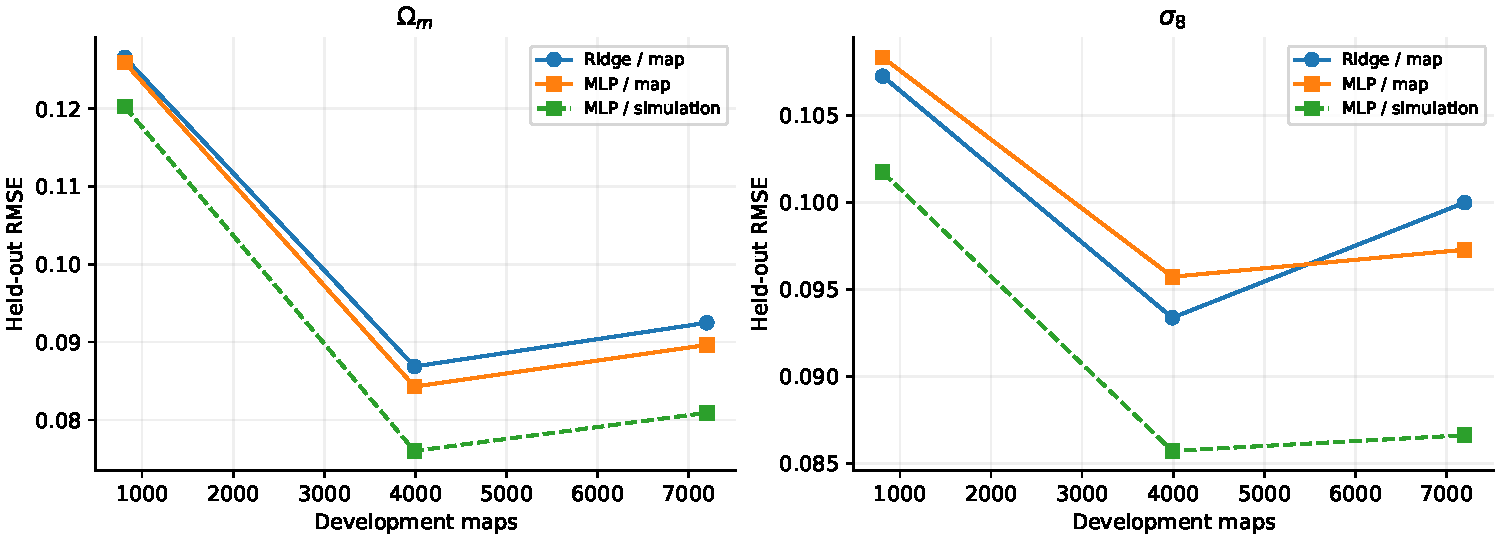
\includegraphics[width=\linewidth]{figures/spectral_comparison.pdf}
\caption{Spectral-model comparison generated from the saved test metrics. Simulation averaging is shown separately from single-map prediction. Levels are disjoint samples rather than nested training subsets.}\label{fig:spectral}
\end{figure}

\begin{figure}[p]\centering
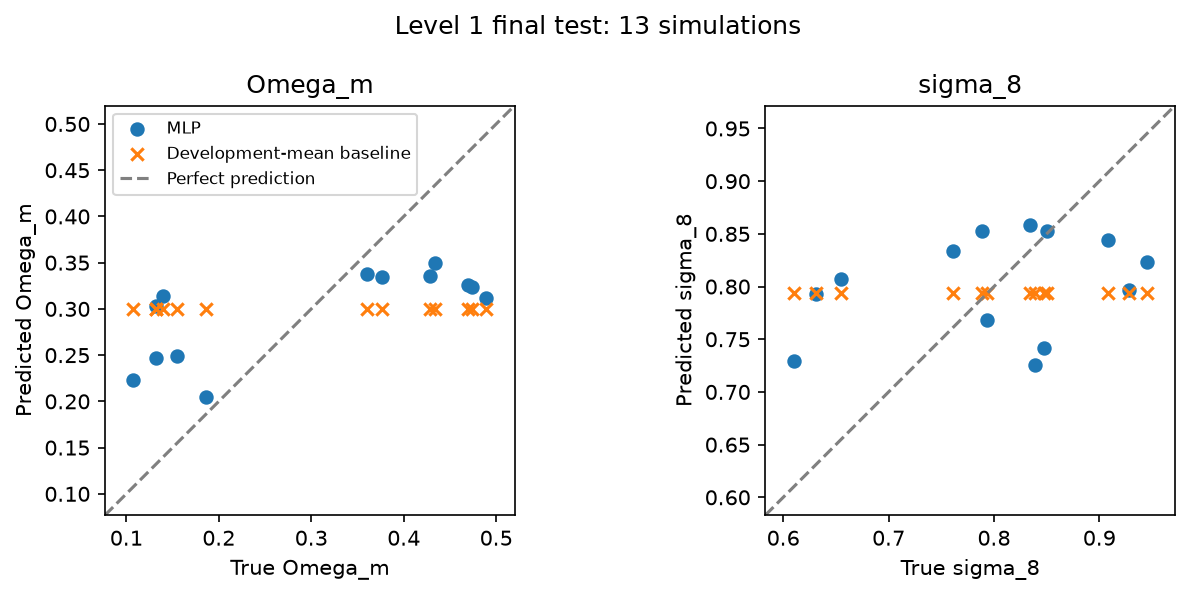
\includegraphics[width=.9\linewidth,height=.22\textheight,keepaspectratio]{figures/mlp_test1.png}\par\vspace{4mm}
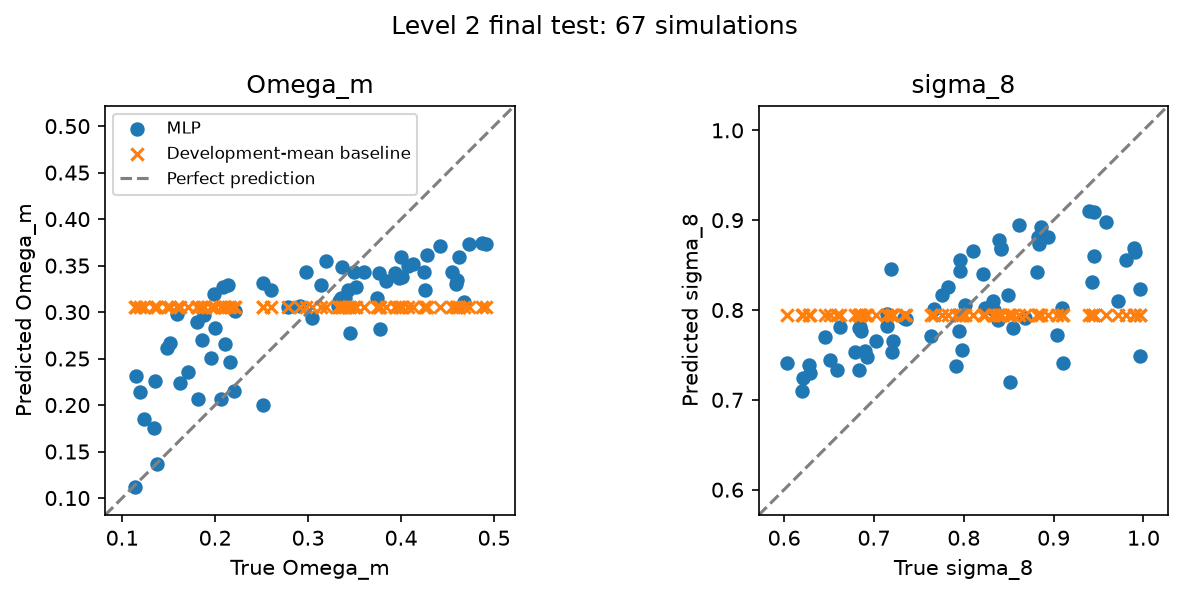
\includegraphics[width=.9\linewidth,height=.22\textheight,keepaspectratio]{figures/mlp_test2.png}\par\vspace{4mm}
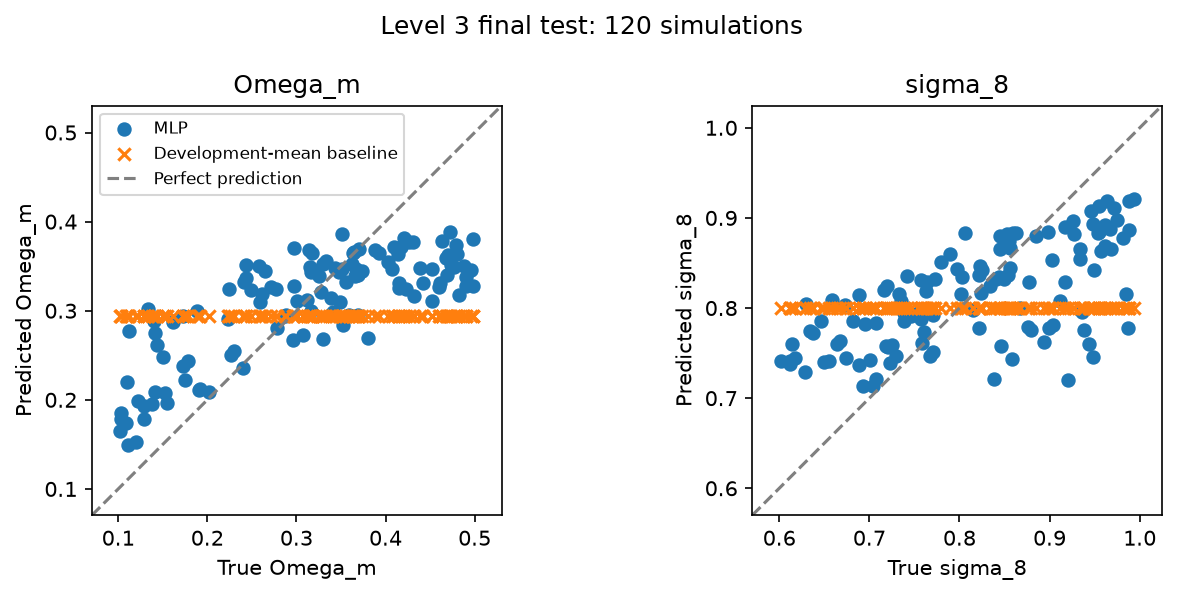
\includegraphics[width=.9\linewidth,height=.22\textheight,keepaspectratio]{figures/mlp_test3.png}
\caption{All saved MLP final test prediction plots, ordered from level 1 (top) to level 3 (bottom). Each point is a simulation-averaged prediction; the baseline predicts the development-target mean.}\label{fig:mlp-tests}
\end{figure}
\FloatBarrier

\section{Results: CNN selection and the common clean test}
\subsection{Validation search}
For the tagged step-4--10 search, the minimum validation MSE changes from 0.0034457 (\model{model_8_5}) at level 1 to 0.0006792 (\model{model_10_5}) at level 2 and 0.0007617 for that same model at level 3. For the tagged step-12--16 search, the winners are \model{model_16_8} at level 1 (0.0011249), \model{model_16_4} at level 2 (0.0005184), and \model{model_16_5} at level 3 (0.0005499). These are validation losses, not held-out test errors.

\begin{figure}[htbp]\centering
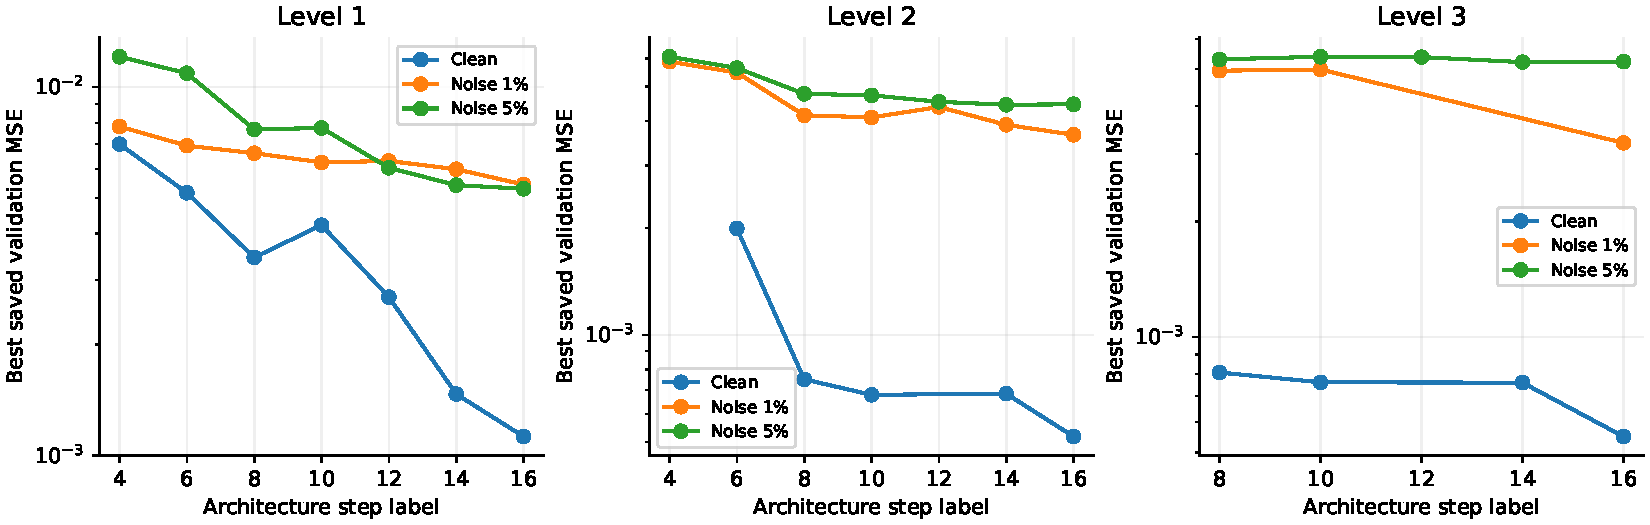
\includegraphics[width=\linewidth]{figures/cnn_validation_summary.pdf}
\caption{Minimum saved validation MSE for each represented step label, level, and corruption setting. Later levels contain shortlisted models, so missing depths were not evaluated there. This plot describes the search record and is not a matched clean-versus-noisy test.}\label{fig:cnn-validation}
\end{figure}

The separate shared files \path{results_level1.json}, \path{results_level2.json}, and \path{results_level3.json} contain 21, ten, and two scores. Their overlapping values differ from the tagged runs; the shared level-3 minimum is 0.0005010 for \model{model_16_4}. The final test workflow explicitly chooses the tagged winners instead. Appendix~\ref{app:cnn} preserves both histories. No shared or tagged score is silently overwritten or combined into one claimed run.

\subsection{Same-test comparison}
\begingroup\footnotesize\setlength{\tabcolsep}{3pt}\renewcommand{\arraystretch}{1.05}
\begin{longtable}{lrrrrrr}
\caption{Common level-3 test comparison: 1,800 maps from 120 held-out simulations; each model was fitted on 7,200 development maps.}\label{tab:common}\\
\toprule
Model & Target & Map RMSE & Map MAE & Sim RMSE & Sim MAE & Map gain \\
\midrule
\endfirsthead
\toprule
Model & Target & Map RMSE & Map MAE & Sim RMSE & Sim MAE & Map gain \\
\midrule\endhead
\bottomrule\endfoot
Ridge & $\Omega_m$ & 0.0925 & 0.0747 & 0.0827 & 0.0675 & 22.8\% \\
Ridge & $\sigma_8$ & 0.1000 & 0.0832 & 0.0940 & 0.0780 & 11.1\% \\
MLP & $\Omega_m$ & 0.0896 & 0.0720 & 0.0809 & 0.0666 & 25.2\% \\
MLP & $\sigma_8$ & 0.0973 & 0.0790 & 0.0866 & 0.0713 & 13.5\% \\
CNN-10 & $\Omega_m$ & 0.0211 & 0.0164 & 0.0111 & 0.0085 & 82.4\% \\
CNN-10 & $\sigma_8$ & 0.0304 & 0.0239 & 0.0161 & 0.0126 & 73.0\% \\
CNN-16 & $\Omega_m$ & 0.0192 & 0.0147 & 0.0106 & 0.0079 & 84.0\% \\
CNN-16 & $\sigma_8$ & 0.0324 & 0.0254 & 0.0245 & 0.0207 & 71.2\% \\
\end{longtable}\endgroup

Both final CNNs substantially outperform the spectral models on the common level-3 test. CNN-16 has the lowest recorded $\Om$ map RMSE, 0.0192, while CNN-10 has the lowest $\sig$ map RMSE, 0.0304. Relative to the common training-mean baseline, those gains are 84.0\% and 73.0\%. Against the MLP's map RMSEs, the reductions are approximately 78.6\% for $\Om$ (CNN-16) and 68.8\% for $\sig$ (CNN-10).

\begin{figure}[htbp]\centering
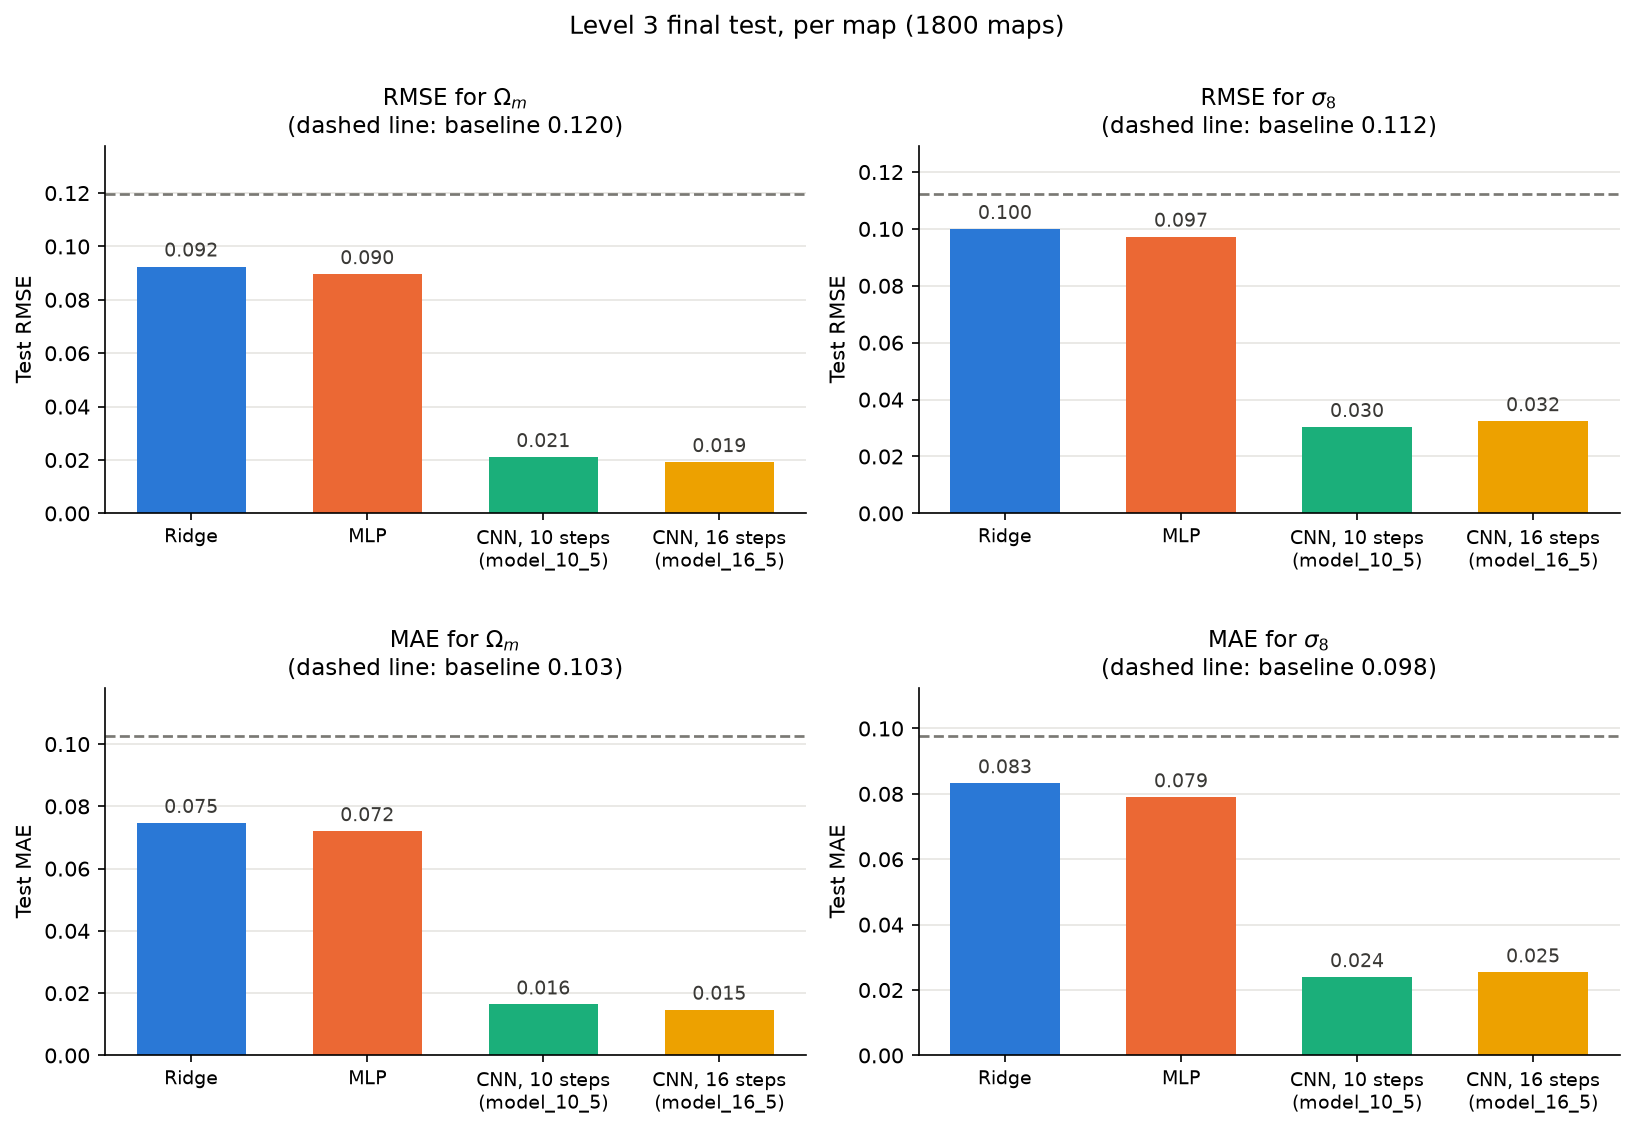
\includegraphics[width=\linewidth]{figures/cnn_errors.png}
\caption{Saved common level-3 map-level RMSE and MAE comparison. The dashed reference is the training-mean baseline. CNN-10 and CNN-16 refer to the fixed final models, not averages over their architecture groups.}\label{fig:cnn-errors}
\end{figure}

\subsection{Simulation averaging and interpretation}
Simulation averaging reduces CNN-10 RMSE to $(0.0111,0.0161)$ and CNN-16 RMSE to $(0.0106,0.0245)$. CNN-16 retains the best $\Om$ score, but CNN-10 is clearly better in the recorded $\sig$ result. The CNN-16 $\sig$ error falls by less under averaging than the CNN-10 error. This is compatible with residual errors shared across views, but the saved aggregate scores alone do not identify their physical cause.

\begin{figure}[p]\centering
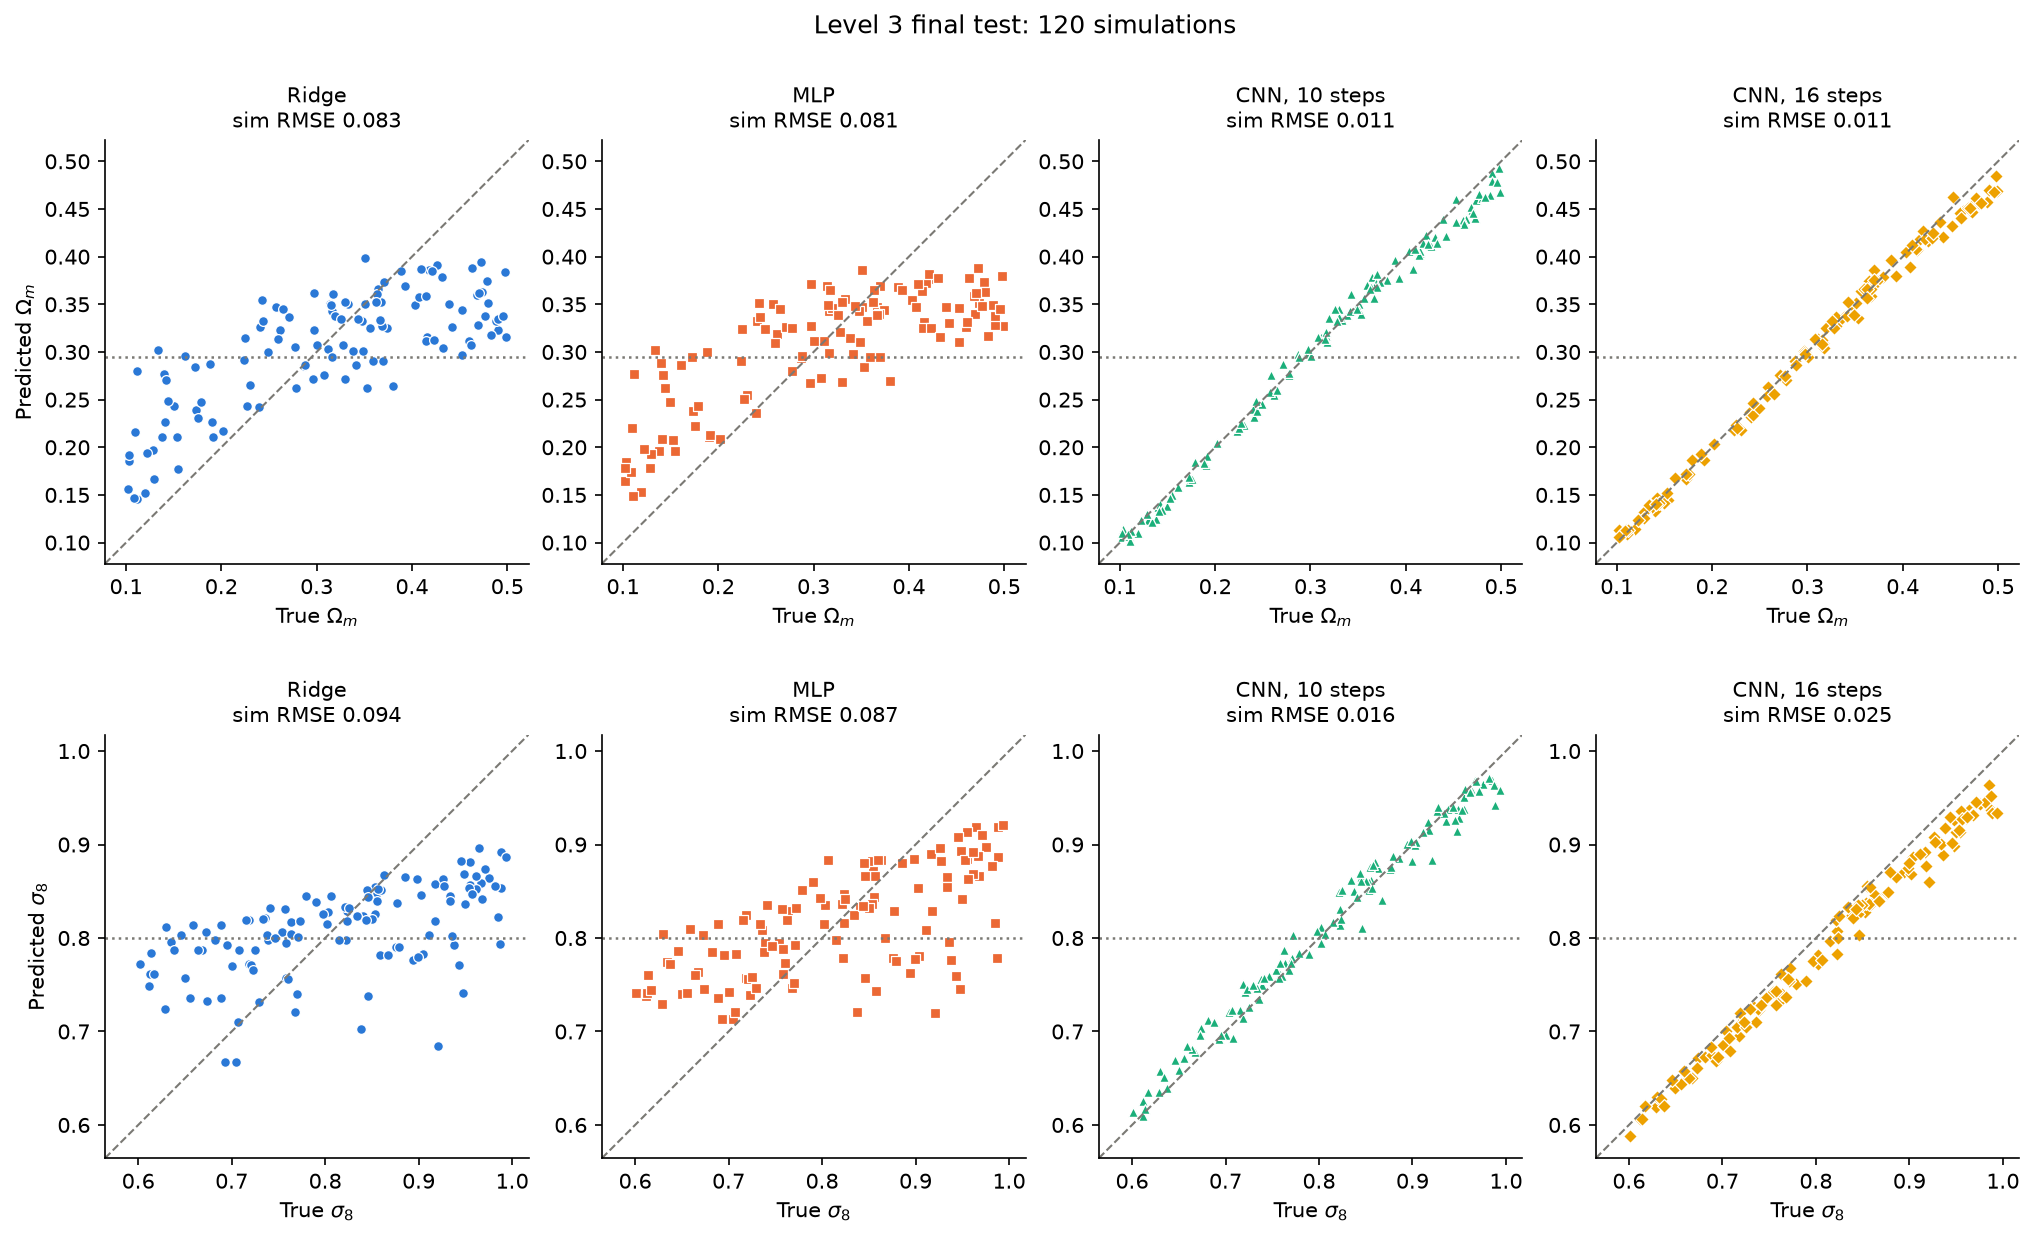
\includegraphics[width=\linewidth,height=.74\textheight,keepaspectratio]{figures/cnn_predictions.png}
\caption{Saved predicted-versus-true comparison for the 120 common test simulations. Each prediction averages 15 map outputs. The CNN predictions lie much closer to the diagonal than the spectral-model predictions.}\label{fig:cnn-predictions}
\end{figure}

The result is consistent with useful information being retained by the spatial representation and learned CNN mapping beyond what these 50-bin spectral regressors extract. It does not isolate a uniquely non-Gaussian physical statistic: input representation, network class, parameter count, optimization, and model-selection procedure all differ. The single-seed CNN outcomes also do not establish that deeper architectures universally improve inference. The target-specific winners show why one should avoid declaring a single architecture best on every criterion.
\FloatBarrier

\section{Results: corrupted-map experiments}
\begingroup\footnotesize\setlength{\tabcolsep}{3pt}\renewcommand{\arraystretch}{1.05}
\begin{longtable}{lrrrrr}
\caption{Saved level-3 noisy-test group averages (five model metrics averaged, not an ensemble). Notebook table precision is six decimals.}\label{tab:noise}\\
\toprule
Group & Noise & MAE $\Omega_m$ & MAE $\sigma_8$ & RMSE $\Omega_m$ & RMSE $\sigma_8$ \\
\midrule
\endfirsthead
\toprule
Group & Noise & MAE $\Omega_m$ & MAE $\sigma_8$ & RMSE $\Omega_m$ & RMSE $\sigma_8$ \\
\midrule\endhead
\bottomrule\endfoot
1 & 1\% Noise & 0.048091 & 0.060267 & 0.060635 & 0.075177 \\
1 & 5\% Noise & 0.050657 & 0.063962 & 0.063642 & 0.080117 \\
2 & 1\% Noise & 0.040007 & 0.053806 & 0.051386 & 0.068414 \\
2 & 5\% Noise & 0.048518 & 0.063897 & 0.061519 & 0.080337 \\
\end{longtable}\endgroup

The saved noisy-test averages increase at the stronger corruption setting for both targets in both groups. Group 1's mean RMSE changes from $(0.060635,0.075177)$ at 1\% noise to $(0.063642,0.080117)$ at 5\% noise. Group 2 changes from $(0.051386,0.068414)$ to $(0.061519,0.080337)$. Group 2 is better on both RMSEs at 1\% noise, but the difference becomes small and target dependent at 5\% noise.

\begin{figure}[p]\centering
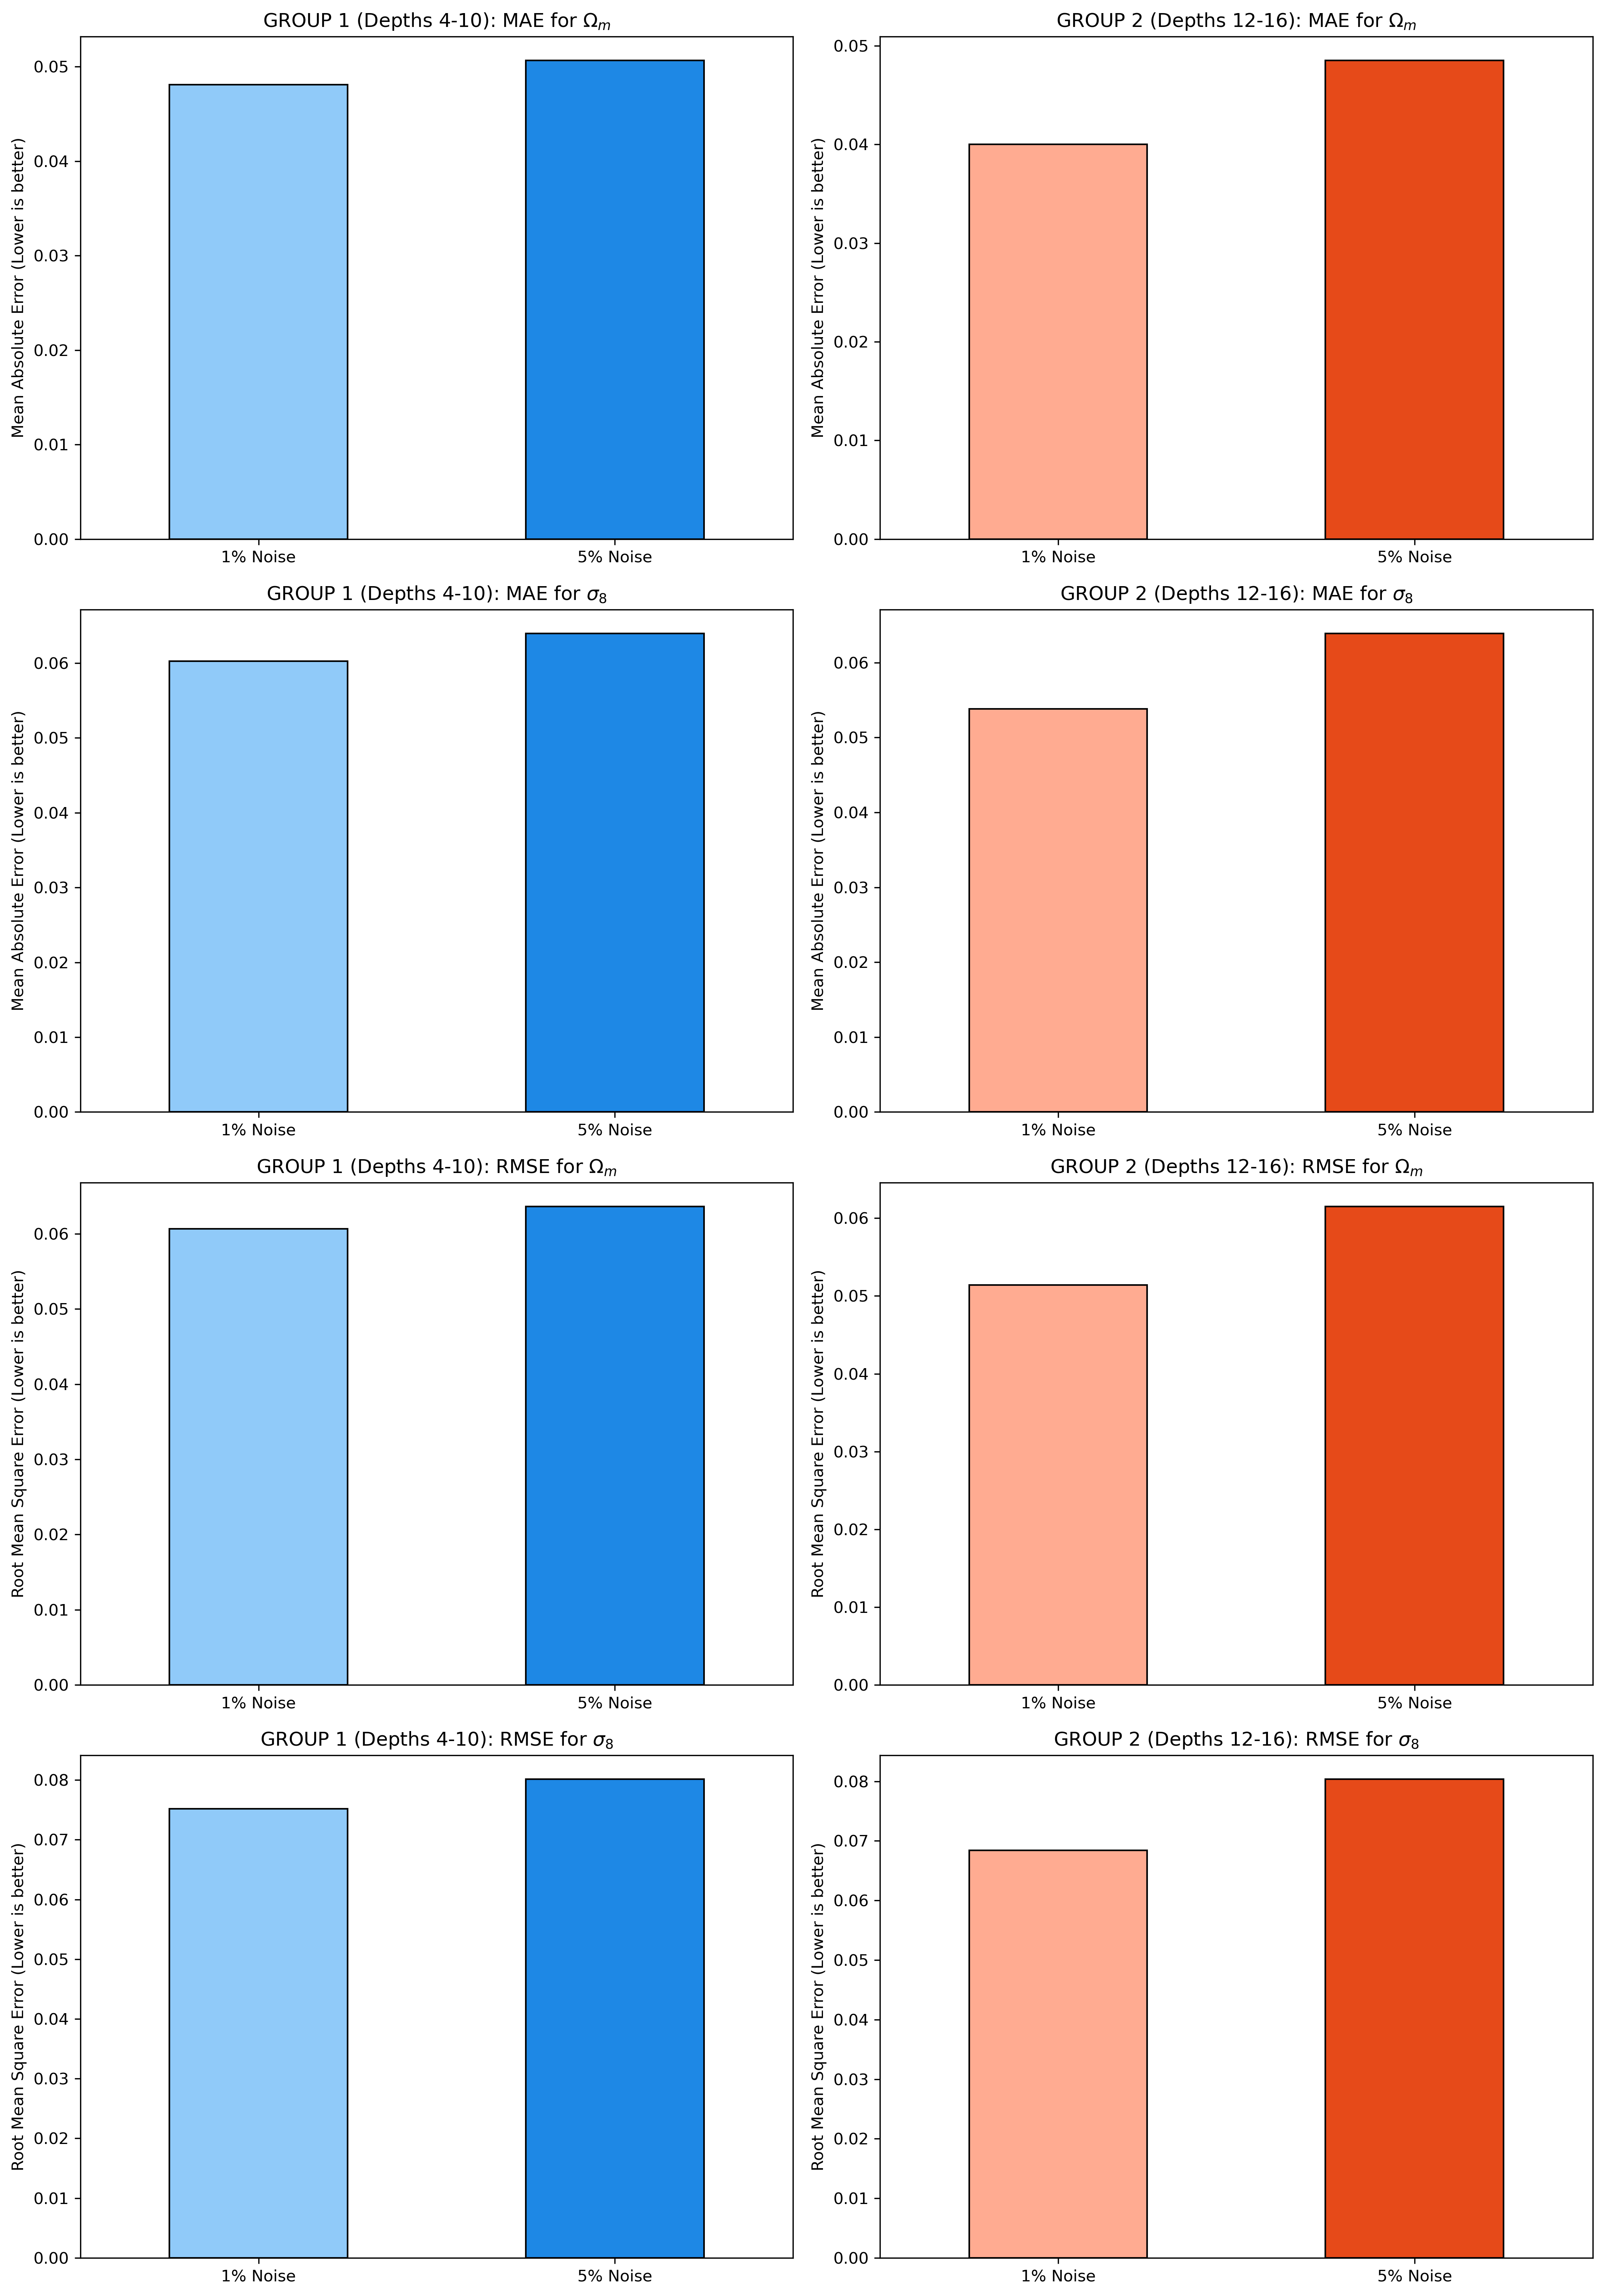
\includegraphics[width=.93\linewidth,height=.78\textheight,keepaspectratio]{figures/augmentation.png}
\caption{Saved eight-panel graph of noisy-test group averages. The bars average metrics from individual checkpoints; they do not measure an ensemble predictor. The clean final test in Table~\ref{tab:common} follows a different fitting protocol.}\label{fig:augmentation}
\end{figure}

All 140 augmented validation scores are retained alongside the 70 tagged clean scores in Appendix~\ref{app:cnn}. The group averages here are taken from the six-decimal tables stored in the notebook, rather than reconstructed from the graph. The notebook's evaluation output contains no printed model failures for this saved run. Its function can skip failed paths, however, and does not store a structured per-model test record or explicit successful-model count, so the group result has less audit detail than the final clean CNN JSON.

These outputs support a limited statement: the saved matched-corruption experiments have higher average errors at $\alpha=0.05$ than at $\alpha=0.01$. They do not quantify robustness of a fixed clean-trained model, establish that Gaussian augmentation improves clean-test generalization, or estimate the causal effect of stronger noise at fixed architecture membership. A decisive follow-up would hold models, training size, and seeds fixed and evaluate a clean/noisy training-by-test matrix, with preprocessing fitted only on the appropriate training data.
\FloatBarrier

\section{Limitations and next experiments}
\subsection{Statistical and scientific limits}
The principal CNN test results come from one seed and one held-out level-3 split after selection on a single validation fold. No repeated-seed variance, simulation-bootstrap confidence intervals, or significance tests are saved. The small test group at level 1 and the disjoint construction of the levels constrain how precisely learning trends can be inferred. MLP cross-validation standard deviations describe development-fold variability, not uncertainty in the final test ranking.

Fifteen correlated maps from the same simulation provide different views, not 15 independent cosmologies. Simulation averaging is useful but presumes access to multiple views at inference. The study is restricted to one field, one redshift, and one simulation suite. It does not evaluate transfer to SIMBA, observational masks, resolution changes, instrumental systematics, posterior calibration, or predictive uncertainty. Consequently, the report claims point-prediction accuracy within the supplied simulated test distribution, not a measurement of the cosmological parameters of the real Universe.

\subsection{Reproducibility and artifact limits}
Historical shared CNN files do not include the settings and provenance needed to reconcile their differences with tagged runs. The original preliminary MLP notebook also has a different batch-order history from the later configuration search. These are preserved as separate evidence, not treated as exact repetitions. The clean final test CSV and the separately saved MLP JSON differ only at small numerical precision: for example, level-3 $\Om$ MLP map RMSE is 0.0896231222 in the common CSV versus 0.0896231011 in its own JSON. Both round to the same values used in this report.

Final MLP JSONs identify checkpoint paths and hashes. Those particular MLP checkpoints are not part of the tracked result set included in this report; the report preserves their metadata and predictions, not a claim that every model can be rerun from this folder alone. The included clean CNN checkpoints in the repository are also not duplicated into the report package. The saved augmentation manifests lack explicit noise provenance, and the repeated leaf seed should be addressed before a controlled robustness experiment.

\subsection{Prioritized follow-up}
The most useful next steps are repeated-seed and simulation-bootstrap comparisons of the two selected CNNs; matched five-fold selection across model families; nested training subsets with a common untouched test set; and a fixed-model clean/noisy evaluation matrix. A stronger spectral baseline or alternative statistics could clarify how much of the CNN advantage comes from information beyond the present compression. Cross-suite testing and calibrated uncertainty estimates would be needed before broader scientific inference claims.

\section{Conclusion}
The saved project results show that both spectral baselines learn some cosmological signal, but their improvements are moderate and $\sig$ inference is weak in the smallest dataset. On the common clean level-3 test, CNNs yield much lower map and simulation errors. CNN-16 leads for $\Om$ while CNN-10 leads for $\sig$, so the recorded evidence favors target-specific assessment over a universal depth ranking. The noise study records worse group-average performance under stronger corruption, while leaving training-time augmentation benefits unresolved. This report retains the full search record, all graphs, and the distinctions necessary to interpret those findings without mixing validation with test performance.

\section{Report provenance and rebuilding}
\label{sec:reproduce}
The report is based on source commit \texttt{\sourcecommit}, captured on 12 November 2026. \path{prepare_report.py} reads the repository's existing outputs, copies evidence to \path{sources/}, extracts notebook images, generates tables and three additional comparison plots, and writes SHA-256 provenance to \path{source_manifest.json}. It never trains a model. Saved CNN map/simulation errors and MLP simulation errors were checked against their stored predictions and targets within absolute tolerance $2\times10^{-7}$.

There are 243 CNN validation records in \path{cnn_scores.csv}: 70 clean tagged, 140 augmented, and 33 historical shared. Seventeen distinct original raster assets are embedded in the document: ten standalone files and seven additional notebook renderings. Identical notebook and standalone images are included once. Three new vector plots summarize existing results without adding experiments. Full-precision structured outputs, notebook text outputs and cell sources, and relevant implementation files are archived beneath \path{sources/}. The source manifest inventories 92 original evidence/code files.

The folder is self-contained for typesetting. From WSL in \path{reports/v1/}, run \texttt{bash build.sh}. The script calls XeLaTeX repeatedly with shell escape disabled, retains the final \path{report.log}, and writes a build-verification summary. It fails on compilation errors, unresolved references/citations, missing characters, or overfull boxes. No bibliography service, external image paths, or Windows-only fonts are required. Regenerating the evidence tables additionally needs the full repository and Python with NumPy, matplotlib, and Pillow.

The repository credits Meirzhan with Ridge regression, Darkhan with the MLP, Danial and Alen with the two CNN groups, and Yeradil with augmentation. The preprocessing README records AI assistance. This report was also assembled with AI assistance from the saved sources; the project team remains responsible for checking its methods, interpretation, and submitted claims.

\begin{thebibliography}{9}
\bibitem{camels} F. Villaescusa-Navarro et al. (2021).
\emph{The CAMELS Project: Cosmology and Astrophysics with Machine-learning Simulations}.
The Astrophysical Journal, 915, 71.
\href{https://doi.org/10.3847/1538-4357/abf7ba}{doi:10.3847/1538-4357/abf7ba}.

\bibitem{cmd} F. Villaescusa-Navarro et al. (2021 preprint).
\emph{The CAMELS Multifield Dataset: Learning the Universe's Fundamental Parameters with Artificial Intelligence}.
\href{https://arxiv.org/abs/2109.10915}{arXiv:2109.10915}.
Published in The Astrophysical Journal Supplement Series (2022), 259, 61,
\href{https://doi.org/10.3847/1538-4365/ac5ab0}{doi:10.3847/1538-4365/ac5ab0}.

\bibitem{docs} CAMELS collaboration.
\emph{CAMELS Multifield Dataset: Description and citation documentation}.
\url{https://camels-multifield-dataset.readthedocs.io/en/latest/data.html};
\url{https://camels-multifield-dataset.readthedocs.io/en/latest/citation.html}.
Accessed 12 November 2026.

\bibitem{repo} CSCI 494 project team.
\emph{Cosmoreg: source code, saved experiment outputs, and notebooks}.
Repository snapshot \texttt{\sourcecommit},
\url{https://github.com/aqalbiat/cosmoreg}.
Original paths, source hashes, and frozen outputs accompany this report in
\path{source_manifest.json} and \path{sources/}.
\end{thebibliography}

\clearpage
\appendix
\section{Complete CNN validation record}
\label{app:cnn}
Tables~\ref{tab:cnn1}--\ref{tab:cnn3} include every model score in the tagged clean and augmented JSONs. An absent score means the model has no saved experiment for that condition and level; it is not an error of zero. The noise-specific shortlists differ, so a row need not contain all three conditions. Values are printed to seven decimal places; \path{cnn_scores.csv} preserves the original numeric precision and source path of each record. Scores average squared errors across both unscaled targets on validation fold 5.

\begingroup\footnotesize\setlength{\tabcolsep}{3pt}\renewcommand{\arraystretch}{1.05}
\begin{longtable}{lrrr}
\caption{All tagged CNN validation scores at level 1; missing experiments are marked with a dash. MSE averages both unscaled targets.}\label{tab:cnn1}\\
\toprule
Model ID & Clean & $\alpha=0.01$ & $\alpha=0.05$ \\
\midrule
\endfirsthead
\toprule
Model ID & Clean & $\alpha=0.01$ & $\alpha=0.05$ \\
\midrule\endhead
\bottomrule\endfoot
model\_4\_1 & 0.0069989 & 0.0141439 & 0.0144408 \\
model\_4\_2 & 0.0082793 & 0.0236685 & 0.0151160 \\
model\_4\_3 & 0.0107882 & 0.0336712 & 0.0146056 \\
model\_4\_4 & 0.0070453 & 0.0078129 & 0.0120850 \\
model\_4\_5 & 0.0073911 & 0.0091129 & 0.0132015 \\
model\_6\_1 & 0.0064164 & 0.0277941 & 0.0174269 \\
model\_6\_2 & 0.0076438 & 0.0194145 & 0.0152957 \\
model\_6\_3 & 0.0058517 & 0.0084581 & 0.0141513 \\
model\_6\_4 & 0.0051821 & 0.0069302 & 0.0109009 \\
model\_6\_5 & 0.0051628 & 0.0070950 & 0.0120668 \\
model\_8\_1 & 0.0054094 & 0.0202418 & 0.0141659 \\
model\_8\_2 & 0.0054884 & 0.0069958 & 0.0121485 \\
model\_8\_3 & 0.0047757 & 0.0096946 & 0.0118738 \\
model\_8\_4 & 0.0045357 & 0.0067857 & 0.0097091 \\
model\_8\_5 & 0.0034457 & 0.0066142 & 0.0076708 \\
model\_10\_1 & 0.0056426 & 0.0121803 & 0.0146704 \\
model\_10\_2 & 0.0058251 & 0.0065384 & 0.0124601 \\
model\_10\_3 & 0.0049765 & 0.0075014 & 0.0117034 \\
model\_10\_4 & 0.0048411 & 0.0062433 & 0.0097992 \\
model\_10\_5 & 0.0042188 & 0.0063721 & 0.0077432 \\
model\_12\_1 & 0.0040244 & 0.0066687 & 0.0100829 \\
model\_12\_2 & 0.0032341 & 0.0062998 & 0.0060358 \\
model\_12\_3 & 0.0026902 & 0.0069767 & 0.0064303 \\
model\_12\_4 & 0.0055355 & 0.0096224 & 0.0138527 \\
model\_12\_5 & 0.0043861 & 0.0070733 & 0.0107536 \\
model\_12\_6 & 0.0029328 & 0.0071253 & 0.0104648 \\
model\_14\_1 & 0.0014673 & 0.0059830 & 0.0054163 \\
model\_14\_2 & 0.0016274 & 0.0066608 & 0.0056889 \\
model\_14\_3 & 0.0105711 & 0.0072500 & 0.0097491 \\
model\_14\_4 & 0.0023917 & 0.0064654 & 0.0063447 \\
model\_14\_5 & 0.0015597 & 0.0061132 & 0.0059752 \\
model\_14\_6 & 0.0018586 & 0.0063835 & 0.0069089 \\
model\_16\_1 & 0.0018689 & 0.0061215 & 0.0053918 \\
model\_16\_2 & 0.0015855 & 0.0054366 & 0.0057412 \\
model\_16\_3 & 0.0016912 & 0.0058233 & 0.0052946 \\
model\_16\_4 & 0.0015311 & 0.0056373 & 0.0054771 \\
model\_16\_5 & 0.0016550 & 0.0059757 & 0.0061370 \\
model\_16\_6 & 0.0017769 & 0.0067787 & 0.0066560 \\
model\_16\_7 & 0.0012060 & 0.0060072 & 0.0053412 \\
model\_16\_8 & 0.0011249 & 0.0059436 & 0.0053472 \\
\end{longtable}\endgroup

\begingroup\footnotesize\setlength{\tabcolsep}{3pt}\renewcommand{\arraystretch}{1.05}
\begin{longtable}{lrrr}
\caption{All tagged CNN validation scores at level 2; missing experiments are marked with a dash. MSE averages both unscaled targets.}\label{tab:cnn2}\\
\toprule
Model ID & Clean & $\alpha=0.01$ & $\alpha=0.05$ \\
\midrule
\endfirsthead
\toprule
Model ID & Clean & $\alpha=0.01$ & $\alpha=0.05$ \\
\midrule\endhead
\bottomrule\endfoot
model\_4\_4 & --- & 0.0058750 & 0.0060658 \\
model\_6\_4 & 0.0019963 & 0.0054757 & 0.0056380 \\
model\_6\_5 & 0.0023349 & 0.0054736 & 0.0063536 \\
model\_8\_1 & 0.0031739 & --- & --- \\
model\_8\_2 & 0.0014938 & 0.0048823 & 0.0052129 \\
model\_8\_3 & 0.0025106 & --- & 0.0073931 \\
model\_8\_4 & 0.0009842 & 0.0044013 & 0.0047704 \\
model\_8\_5 & 0.0007510 & 0.0041515 & 0.0048007 \\
model\_10\_2 & --- & 0.0048594 & --- \\
model\_10\_3 & 0.0021099 & 0.0052358 & 0.0068009 \\
model\_10\_4 & 0.0011107 & 0.0045545 & 0.0048500 \\
model\_10\_5 & 0.0006792 & 0.0040968 & 0.0047251 \\
model\_12\_2 & --- & 0.0043813 & 0.0045310 \\
model\_14\_1 & 0.0007392 & 0.0041115 & 0.0054247 \\
model\_14\_2 & 0.0006843 & --- & 0.0044436 \\
model\_14\_5 & 0.0007257 & 0.0039031 & 0.0050467 \\
model\_16\_1 & --- & 0.0038774 & 0.0046204 \\
model\_16\_2 & 0.0007366 & 0.0038953 & 0.0046253 \\
model\_16\_3 & 0.0006844 & 0.0036855 & 0.0052517 \\
model\_16\_4 & 0.0005184 & 0.0036595 & 0.0047026 \\
model\_16\_5 & 0.0007064 & 0.0037948 & --- \\
model\_16\_6 & 0.0008488 & --- & --- \\
model\_16\_7 & 0.0006844 & 0.0039826 & 0.0044587 \\
model\_16\_8 & 0.0007591 & 0.0041321 & 0.0049695 \\
\end{longtable}\endgroup

\begingroup\footnotesize\setlength{\tabcolsep}{3pt}\renewcommand{\arraystretch}{1.05}
\begin{longtable}{lrrr}
\caption{All tagged CNN validation scores at level 3; missing experiments are marked with a dash. MSE averages both unscaled targets.}\label{tab:cnn3}\\
\toprule
Model ID & Clean & $\alpha=0.01$ & $\alpha=0.05$ \\
\midrule
\endfirsthead
\toprule
Model ID & Clean & $\alpha=0.01$ & $\alpha=0.05$ \\
\midrule\endhead
\bottomrule\endfoot
model\_8\_2 & 0.0013124 & --- & 0.0056304 \\
model\_8\_4 & 0.0009603 & 0.0051284 & 0.0053509 \\
model\_8\_5 & 0.0008078 & 0.0049506 & 0.0052993 \\
model\_10\_2 & --- & 0.0055163 & --- \\
model\_10\_4 & 0.0010026 & 0.0051077 & 0.0054504 \\
model\_10\_5 & 0.0007617 & 0.0049868 & 0.0053833 \\
model\_12\_2 & --- & --- & 0.0053718 \\
model\_14\_2 & 0.0007600 & --- & 0.0052118 \\
model\_16\_1 & --- & 0.0045318 & 0.0052257 \\
model\_16\_2 & --- & 0.0036096 & 0.0055995 \\
model\_16\_3 & 0.0006406 & 0.0035592 & --- \\
model\_16\_4 & 0.0005674 & 0.0033524 & --- \\
model\_16\_5 & 0.0005499 & 0.0032087 & --- \\
model\_16\_7 & 0.0006502 & --- & 0.0057286 \\
\end{longtable}\endgroup


\subsection{Historical shared-file scores}
The following shared-file values are retained separately because overlapping models have different saved results and incomplete run metadata. In particular, the shared file includes an older \model{model_1} score not present in the current registry. These values are not used to replace the tagged winners in the final clean-test narrative.
\begingroup\footnotesize\setlength{\tabcolsep}{3pt}\renewcommand{\arraystretch}{1.05}
\begin{longtable}{lrrr}
\caption{Separate historical shared-file CNN scores. These are preserved rather than substituted for the tagged runs used by the final-selection workflow.}\label{tab:cnn-shared}\\
\toprule
Model ID & Level 1 & Level 2 & Level 3 \\
\midrule
\endfirsthead
\toprule
Model ID & Level 1 & Level 2 & Level 3 \\
\midrule\endhead
\bottomrule\endfoot
model\_1 & 0.0057940 & --- & --- \\
model\_12\_1 & 0.0040243 & --- & --- \\
model\_12\_2 & 0.0032314 & --- & --- \\
model\_12\_3 & 0.0026914 & --- & --- \\
model\_12\_4 & 0.0055486 & --- & --- \\
model\_12\_5 & 0.0043861 & --- & --- \\
model\_12\_6 & 0.0029329 & --- & --- \\
model\_14\_1 & 0.0014662 & 0.0006376 & --- \\
model\_14\_2 & 0.0016288 & 0.0006363 & --- \\
model\_14\_3 & 0.0099492 & --- & --- \\
model\_14\_4 & 0.0023833 & --- & --- \\
model\_14\_5 & 0.0016164 & 0.0006647 & --- \\
model\_14\_6 & 0.0018610 & --- & --- \\
model\_16\_1 & 0.0018855 & --- & --- \\
model\_16\_2 & 0.0016104 & 0.0006102 & 0.0006250 \\
model\_16\_3 & 0.0017112 & 0.0006665 & --- \\
model\_16\_4 & 0.0014847 & 0.0005327 & 0.0005010 \\
model\_16\_5 & 0.0016477 & 0.0006477 & --- \\
model\_16\_6 & 0.0018126 & 0.0008026 & --- \\
model\_16\_7 & 0.0011943 & 0.0006364 & --- \\
model\_16\_8 & 0.0011175 & 0.0006850 & --- \\
\end{longtable}\endgroup


\clearpage
\section{Complete MLP configuration/fold record}
\label{app:mlp}
The following table covers all three configurations, five validation folds, and three levels. The loss column is standardized-target MSE at the retained epoch. RMSE and MAE are evaluated after averaging predictions by simulation, in original units. Per-fold map metrics, baseline metrics, settings, and full training/validation histories remain available at their original precision in the archived configuration-comparison JSONs. Final training durations and checkpoint metadata remain in the archived final-selection and test-result files.
\begingroup\footnotesize\setlength{\tabcolsep}{3pt}\renewcommand{\arraystretch}{1.05}
\begin{longtable}{lrrrrrrrr}
\caption{All 45 MLP configuration/fold experiments, with simulation-level errors in original units.}\label{tab:mlp-folds}\\
\toprule
Level & Configuration & Fold & Epoch & Std MSE & RMSE $\Omega_m$ & RMSE $\sigma_8$ & MAE $\Omega_m$ & MAE $\sigma_8$ \\
\midrule
\endfirsthead
\toprule
Level & Configuration & Fold & Epoch & Std MSE & RMSE $\Omega_m$ & RMSE $\sigma_8$ & MAE $\Omega_m$ & MAE $\sigma_8$ \\
\midrule\endhead
\bottomrule\endfoot
1 & original & 1 & 9 & 0.4173 & 0.0708 & 0.0619 & 0.0599 & 0.0544 \\
1 & original & 2 & 17 & 0.7438 & 0.0799 & 0.0946 & 0.0633 & 0.0803 \\
1 & original & 3 & 18 & 1.0849 & 0.0977 & 0.1063 & 0.0923 & 0.0920 \\
1 & original & 4 & 11 & 0.5755 & 0.0780 & 0.0771 & 0.0591 & 0.0616 \\
1 & original & 5 & 20 & 1.1611 & 0.1150 & 0.1037 & 0.1064 & 0.0926 \\
1 & larger & 1 & 3 & 0.3941 & 0.0694 & 0.0584 & 0.0583 & 0.0512 \\
1 & larger & 2 & 6 & 0.7480 & 0.0794 & 0.0968 & 0.0654 & 0.0824 \\
1 & larger & 3 & 18 & 1.0331 & 0.0928 & 0.1057 & 0.0871 & 0.0918 \\
1 & larger & 4 & 11 & 0.5734 & 0.0754 & 0.0790 & 0.0582 & 0.0653 \\
1 & larger & 5 & 19 & 1.1275 & 0.1132 & 0.1029 & 0.1040 & 0.0919 \\
1 & stronger\_decay & 1 & 9 & 0.4188 & 0.0710 & 0.0620 & 0.0602 & 0.0546 \\
1 & stronger\_decay & 2 & 17 & 0.7454 & 0.0801 & 0.0946 & 0.0635 & 0.0802 \\
1 & stronger\_decay & 3 & 18 & 1.0869 & 0.0978 & 0.1065 & 0.0923 & 0.0922 \\
1 & stronger\_decay & 4 & 11 & 0.5761 & 0.0781 & 0.0771 & 0.0591 & 0.0617 \\
1 & stronger\_decay & 5 & 20 & 1.1611 & 0.1151 & 0.1037 & 0.1064 & 0.0926 \\
2 & original & 1 & 13 & 0.5941 & 0.0772 & 0.0763 & 0.0656 & 0.0635 \\
2 & original & 2 & 13 & 0.6978 & 0.0802 & 0.0888 & 0.0696 & 0.0736 \\
2 & original & 3 & 19 & 0.5878 & 0.0749 & 0.0795 & 0.0643 & 0.0663 \\
2 & original & 4 & 12 & 0.7356 & 0.0864 & 0.0867 & 0.0746 & 0.0735 \\
2 & original & 5 & 13 & 0.4926 & 0.0715 & 0.0703 & 0.0599 & 0.0594 \\
2 & larger & 1 & 17 & 0.5977 & 0.0791 & 0.0760 & 0.0673 & 0.0634 \\
2 & larger & 2 & 13 & 0.6953 & 0.0785 & 0.0893 & 0.0674 & 0.0750 \\
2 & larger & 3 & 17 & 0.5791 & 0.0745 & 0.0799 & 0.0638 & 0.0672 \\
2 & larger & 4 & 5 & 0.7276 & 0.0869 & 0.0866 & 0.0751 & 0.0731 \\
2 & larger & 5 & 13 & 0.4898 & 0.0716 & 0.0695 & 0.0594 & 0.0590 \\
2 & stronger\_decay & 1 & 13 & 0.5948 & 0.0773 & 0.0764 & 0.0657 & 0.0636 \\
2 & stronger\_decay & 2 & 13 & 0.6958 & 0.0800 & 0.0888 & 0.0695 & 0.0737 \\
2 & stronger\_decay & 3 & 19 & 0.5875 & 0.0747 & 0.0799 & 0.0641 & 0.0668 \\
2 & stronger\_decay & 4 & 11 & 0.7359 & 0.0868 & 0.0864 & 0.0752 & 0.0731 \\
2 & stronger\_decay & 5 & 13 & 0.4911 & 0.0710 & 0.0702 & 0.0594 & 0.0594 \\
3 & original & 1 & 12 & 0.5819 & 0.0784 & 0.0805 & 0.0663 & 0.0682 \\
3 & original & 2 & 18 & 0.5908 & 0.0749 & 0.0881 & 0.0631 & 0.0730 \\
3 & original & 3 & 16 & 0.6369 & 0.0805 & 0.0879 & 0.0683 & 0.0752 \\
3 & original & 4 & 9 & 0.5919 & 0.0787 & 0.0814 & 0.0662 & 0.0717 \\
3 & original & 5 & 17 & 0.7073 & 0.0855 & 0.0898 & 0.0731 & 0.0749 \\
3 & larger & 1 & 12 & 0.5766 & 0.0778 & 0.0805 & 0.0659 & 0.0683 \\
3 & larger & 2 & 16 & 0.5841 & 0.0711 & 0.0869 & 0.0583 & 0.0714 \\
3 & larger & 3 & 9 & 0.6345 & 0.0803 & 0.0861 & 0.0684 & 0.0734 \\
3 & larger & 4 & 4 & 0.5983 & 0.0796 & 0.0823 & 0.0666 & 0.0721 \\
3 & larger & 5 & 17 & 0.7059 & 0.0848 & 0.0898 & 0.0719 & 0.0747 \\
3 & stronger\_decay & 1 & 12 & 0.5811 & 0.0786 & 0.0804 & 0.0665 & 0.0681 \\
3 & stronger\_decay & 2 & 18 & 0.5900 & 0.0749 & 0.0881 & 0.0630 & 0.0730 \\
3 & stronger\_decay & 3 & 16 & 0.6373 & 0.0810 & 0.0879 & 0.0688 & 0.0752 \\
3 & stronger\_decay & 4 & 9 & 0.5916 & 0.0790 & 0.0814 & 0.0667 & 0.0718 \\
3 & stronger\_decay & 5 & 19 & 0.7071 & 0.0842 & 0.0901 & 0.0702 & 0.0751 \\
\end{longtable}\endgroup


\clearpage
\section{Figure inventory and original notebook renderings}
\label{app:figures}
All ten standalone raster graphs appear in the main report. Seven further notebook renderings have different file hashes, generally reflecting export resolution or layout, and are preserved on the following pages. They depict the same experiment families and must not be counted as additional experiments. The three MLP test notebook images are byte-identical to their standalone versions and are included once. Notebook cell numbers are zero based. The full inventory below maps every original raster asset to its repository source.
\begingroup\footnotesize\setlength{\tabcolsep}{3pt}\renewcommand{\arraystretch}{1.05}
\begin{longtable}{p{.39\linewidth}p{.55\linewidth}}
\caption{Inventory of all original saved raster graphs, including distinct notebook renderings.}\label{tab:figures}\\
\toprule
Report asset & Original source \\
\midrule
\endfirsthead
\toprule
Report asset & Original source \\
\midrule\endhead
\bottomrule\endfoot
\path{ridge_cv.png} & \path{results/ridge/cv_curves.png} \\
\path{ridge_predictions.png} & \path{results/ridge/pred_vs_true.png} \\
\path{ridge_size.png} & \path{results/ridge/rmse_vs_train_size.png} \\
\path{mlp_learning.png} & \path{mlp/level1/mlp_learning_curves.png} \\
\path{mlp_test1.png} & \path{mlp/level1/level1_test_predictions.png} \\
\path{mlp_test2.png} & \path{mlp/level2/level2_test_predictions.png} \\
\path{mlp_test3.png} & \path{mlp/level3/level3_test_predictions.png} \\
\path{cnn_errors.png} & \path{cnn_test/level3_test_errors.png} \\
\path{cnn_predictions.png} & \path{cnn_test/level3_test_predictions.png} \\
\path{augmentation.png} & \path{augment/Group_Comparison_Noise_Complete.png} \\
\path{nb_compare_results_c3_o0.png} & \path{augment/compare_results.ipynb} (cell 3) \\
\path{nb_cnn_test_c12_o0.png} & \path{cnn_test/cnn_test.ipynb} (cell 12) \\
\path{nb_cnn_test_c14_o0.png} & \path{cnn_test/cnn_test.ipynb} (cell 14) \\
\path{nb_mlp_validation_c28_o0.png} & \path{mlp/level1/mlp_validation.ipynb} (cell 28) \\
\path{nb_ridge_c8_o0.png} & \path{ridge.ipynb} (cell 8) \\
\path{nb_ridge_c11_o0.png} & \path{ridge.ipynb} (cell 11) \\
\path{nb_ridge_c12_o0.png} & \path{ridge.ipynb} (cell 12) \\
\end{longtable}\endgroup

\clearpage
\begin{figure}[p]\centering
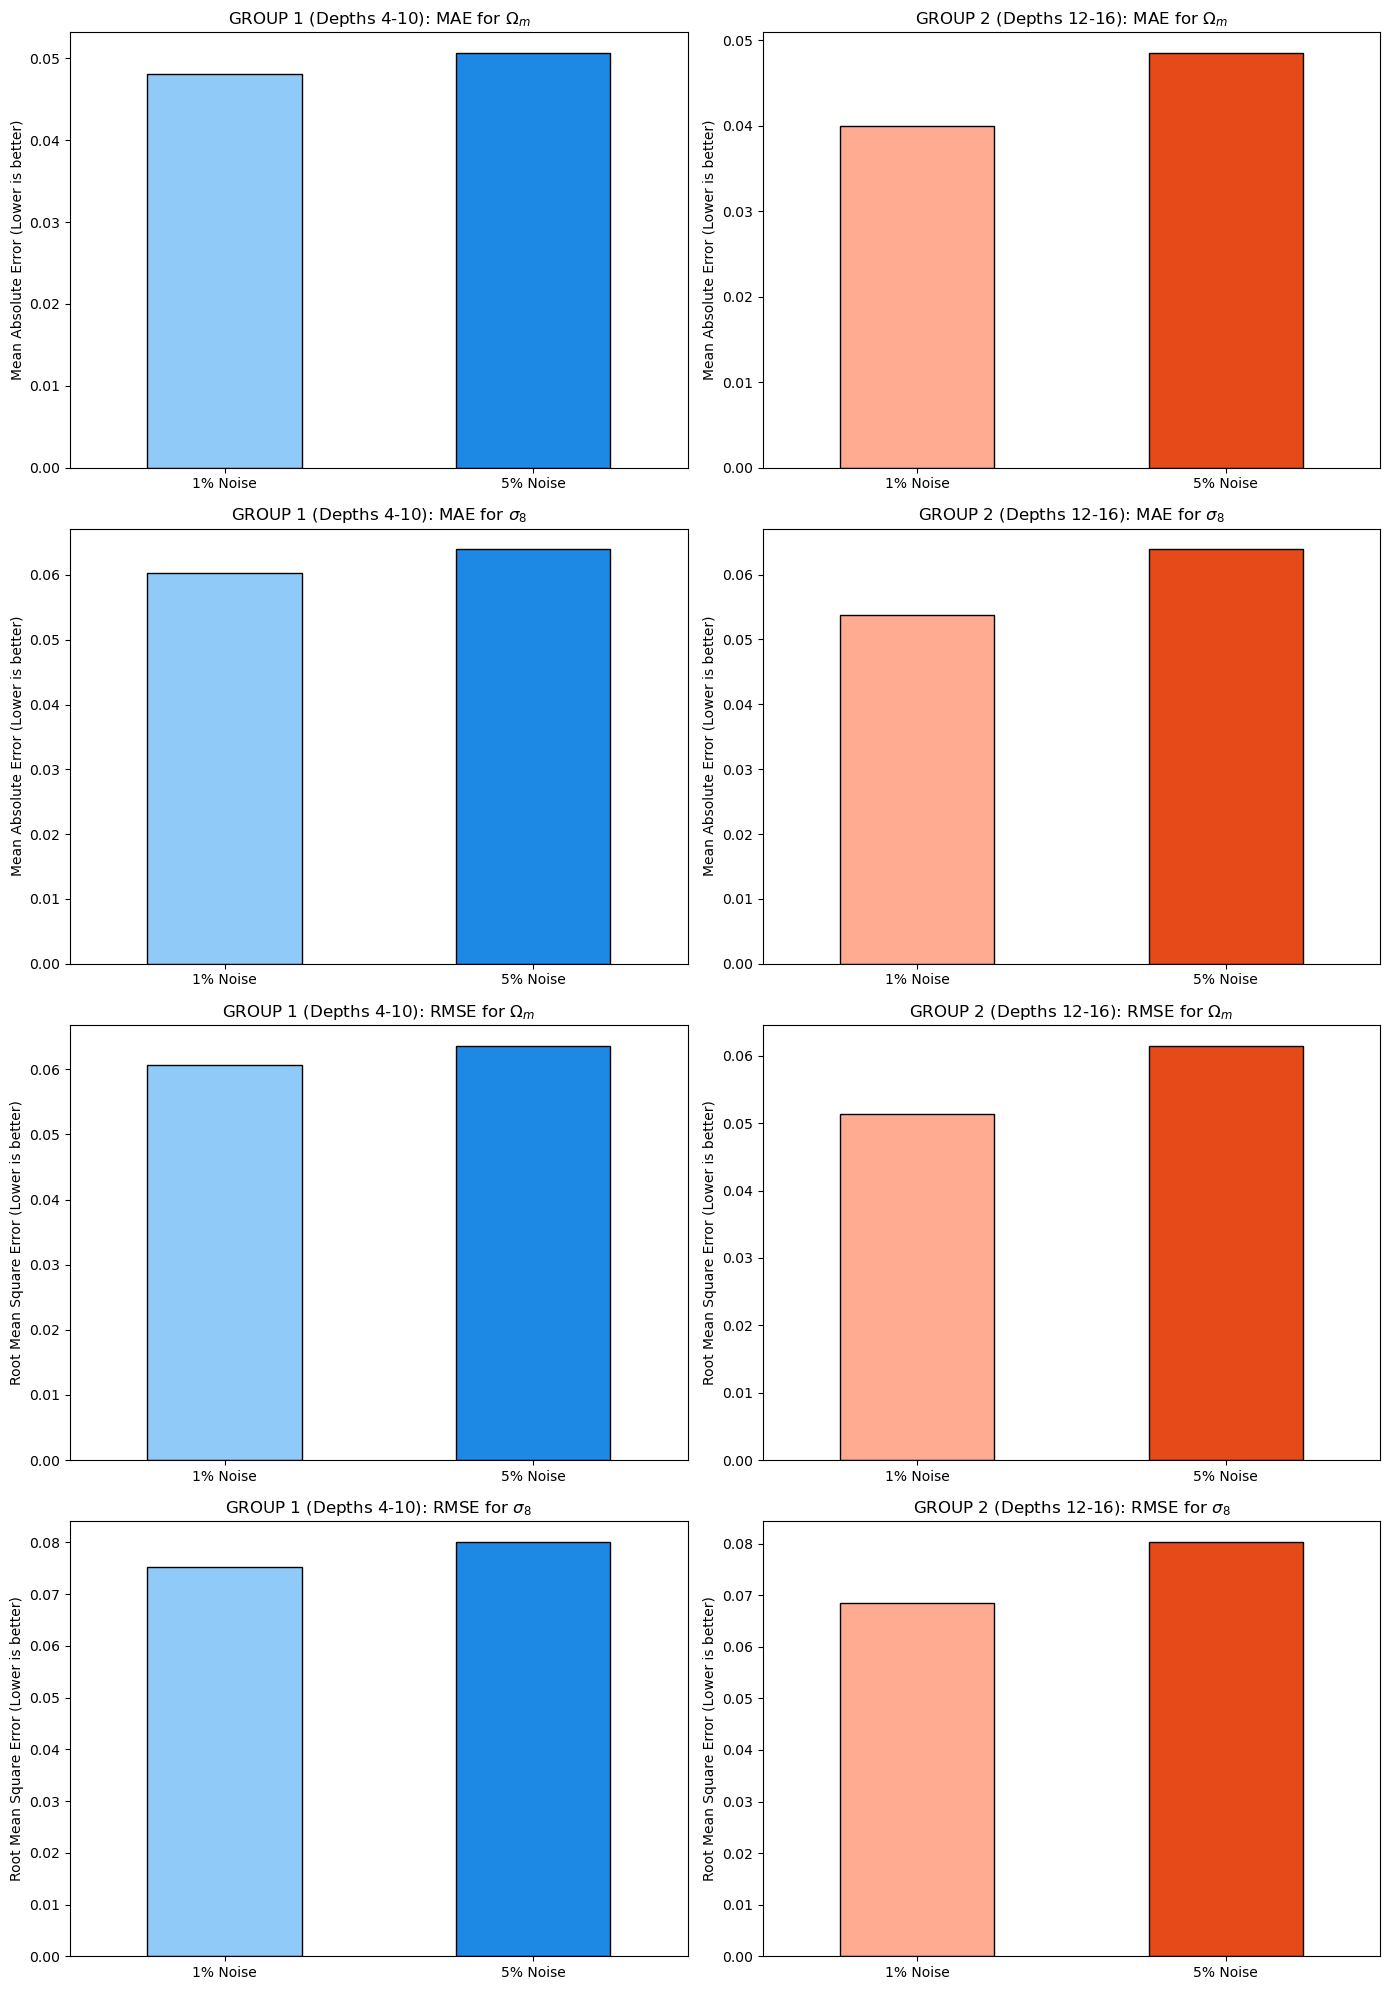
\includegraphics[width=.92\linewidth,height=.72\textheight,keepaspectratio]{figures/nb_compare_results_c3_o0.png}
\caption{Embedded notebook rendering from \texttt{augment/compare\_results.ipynb}, cell 3 (zero based). This preserves the notebook's saved version of the plot.}
\end{figure}\clearpage
\begin{figure}[p]\centering
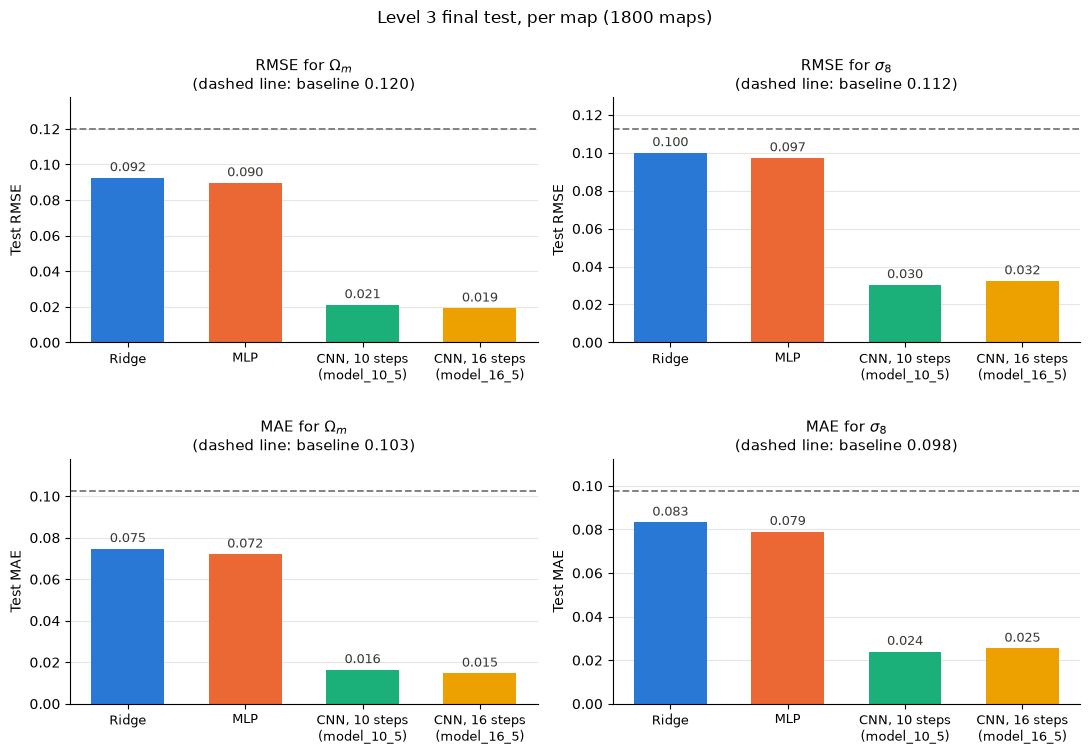
\includegraphics[width=.92\linewidth,height=.72\textheight,keepaspectratio]{figures/nb_cnn_test_c12_o0.png}
\caption{Embedded notebook rendering from \texttt{cnn\_test/cnn\_test.ipynb}, cell 12 (zero based). This preserves the notebook's saved version of the plot.}
\end{figure}\clearpage
\begin{figure}[p]\centering
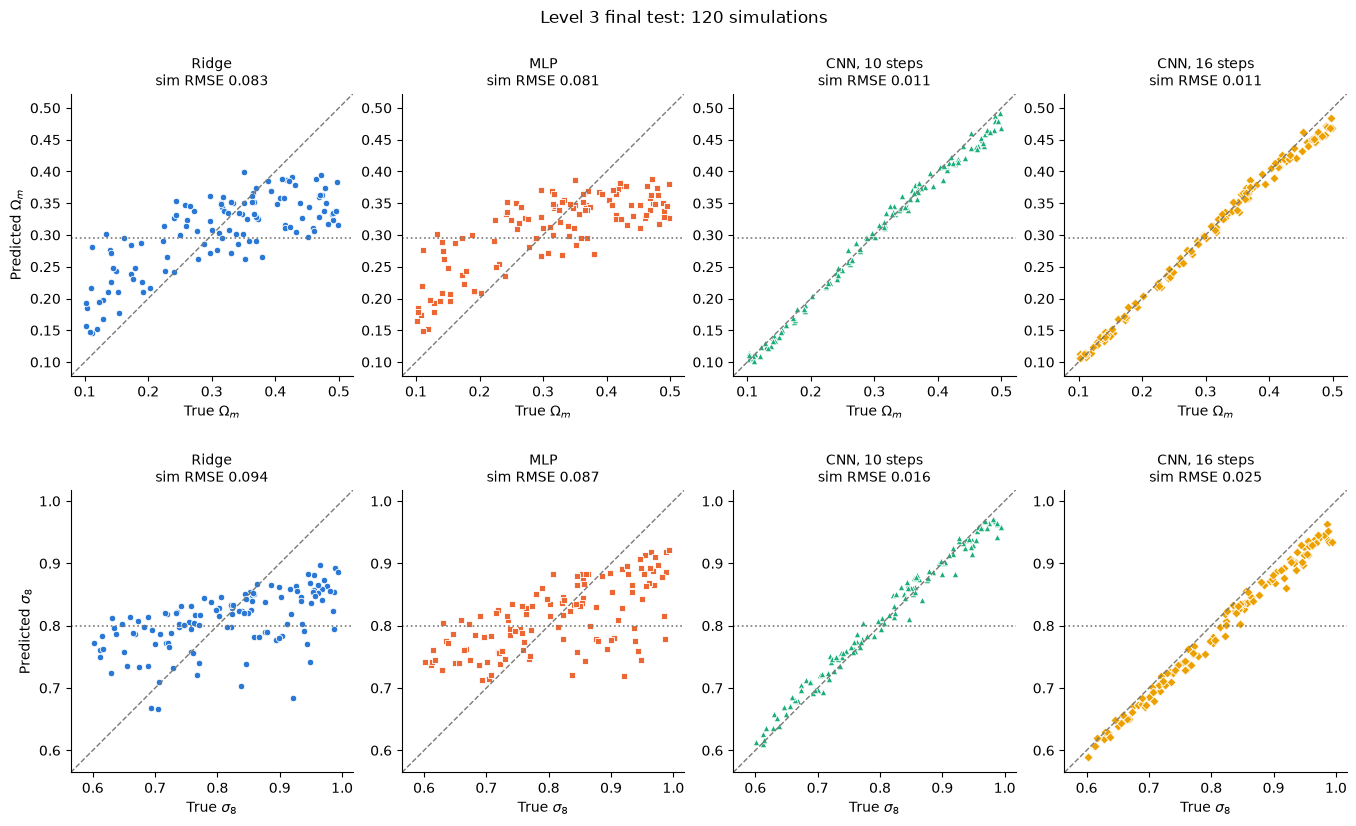
\includegraphics[width=.92\linewidth,height=.72\textheight,keepaspectratio]{figures/nb_cnn_test_c14_o0.png}
\caption{Embedded notebook rendering from \texttt{cnn\_test/cnn\_test.ipynb}, cell 14 (zero based). This preserves the notebook's saved version of the plot.}
\end{figure}\clearpage
\begin{figure}[p]\centering
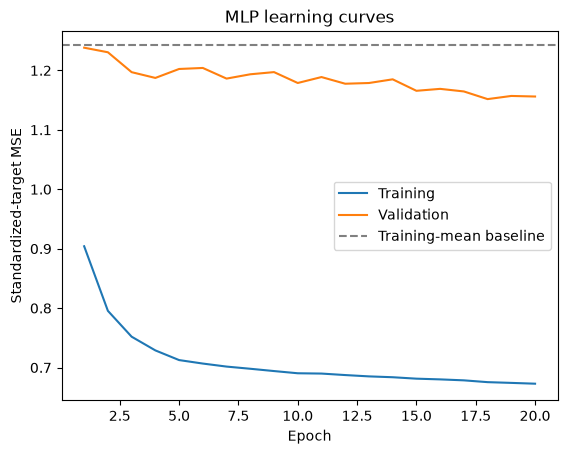
\includegraphics[width=.92\linewidth,height=.72\textheight,keepaspectratio]{figures/nb_mlp_validation_c28_o0.png}
\caption{Embedded notebook rendering from \texttt{mlp/level1/mlp\_validation.ipynb}, cell 28 (zero based). This preserves the notebook's saved version of the plot.}
\end{figure}\clearpage
\begin{figure}[p]\centering
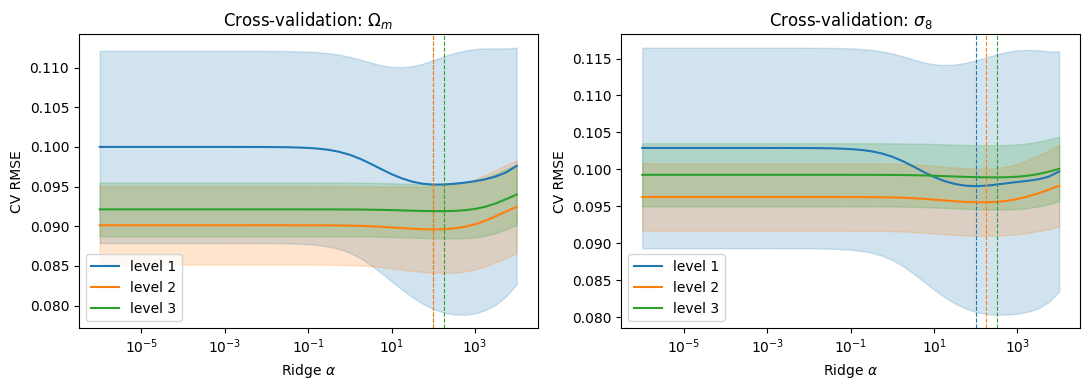
\includegraphics[width=.92\linewidth,height=.72\textheight,keepaspectratio]{figures/nb_ridge_c8_o0.png}
\caption{Embedded notebook rendering from \texttt{ridge.ipynb}, cell 8 (zero based). This preserves the notebook's saved version of the plot.}
\end{figure}\clearpage
\begin{figure}[p]\centering
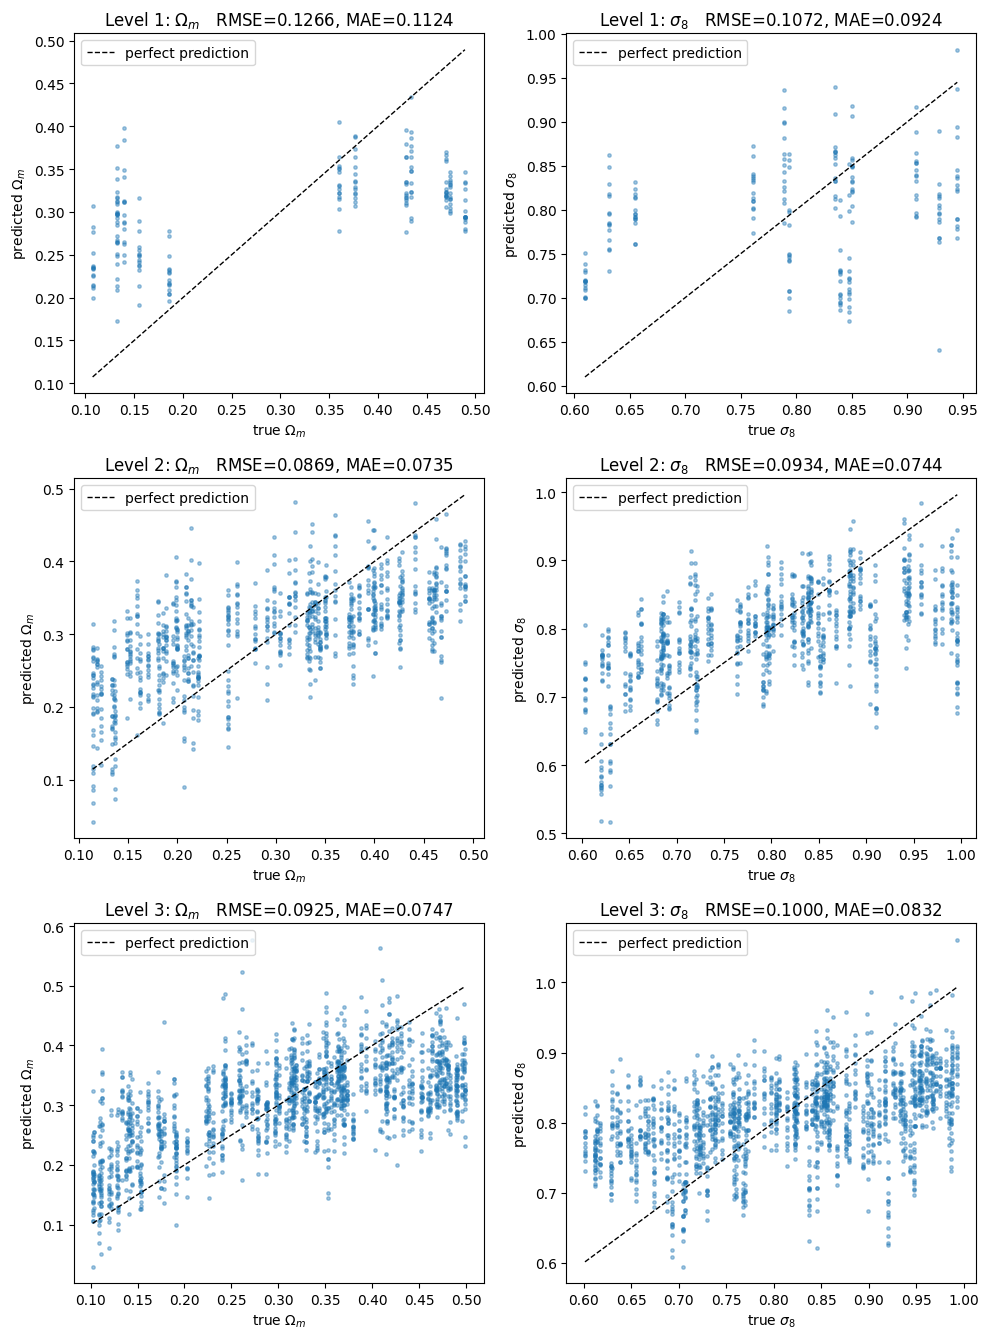
\includegraphics[width=.92\linewidth,height=.72\textheight,keepaspectratio]{figures/nb_ridge_c11_o0.png}
\caption{Embedded notebook rendering from \texttt{ridge.ipynb}, cell 11 (zero based). This preserves the notebook's saved version of the plot.}
\end{figure}\clearpage
\begin{figure}[p]\centering
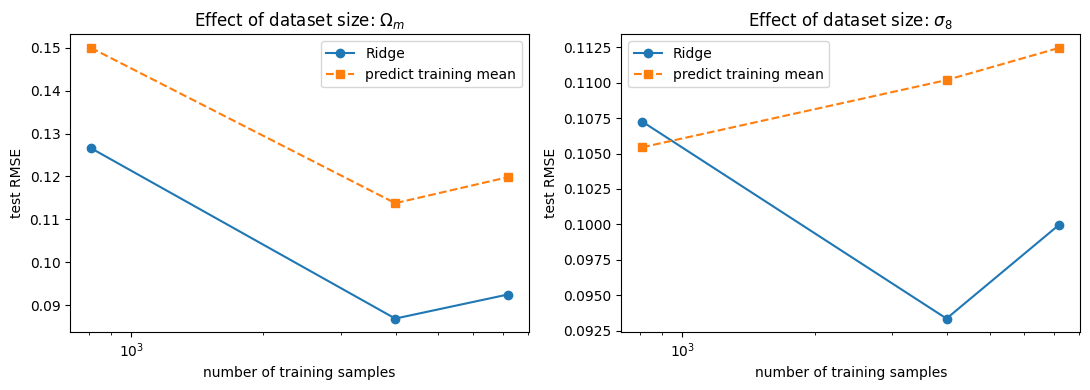
\includegraphics[width=.92\linewidth,height=.72\textheight,keepaspectratio]{figures/nb_ridge_c12_o0.png}
\caption{Embedded notebook rendering from \texttt{ridge.ipynb}, cell 12 (zero based). This preserves the notebook's saved version of the plot.}
\end{figure}\clearpage
\end{document}
